\documentclass[letterpaper]{report}

\usepackage{polyglossia}
\setdefaultlanguage{spanish}



%\usepackage[spanish]{babel}
%\usepackage[utf8]{inputenc}

\usepackage{graphicx}
\usepackage{footnote}
\usepackage[top=2.5cm, left=3cm, right=3cm, bottom=2.5cm]{geometry}

\linespread{1.5}

\setlength{\parskip}{2ex}
\parindent 3ex

\usepackage[backend=biber,sorting=none]{biblatex}
\bibliography{Bibliografia/biblio}

\usepackage[linktocpage=true,hidelinks]{hyperref}

\DeclareGraphicsExtensions{.jpg,.pdf,.png}

\begin{document}	
     
     % Portada
%     \begin{titlepage}
    \begin{center}
        
        % Upper part
        
\includegraphics[scale=0.5]{figures/logo} \\
        
        \textsc {\large UNIVERSIDAD SIM\'ON BOL\'IVAR} \\
        \textsc{DECANATO DE ESTUDIOS PROFESIONALES\\
            COORDINACI\'ON DE INGENIER\'IA DE LA COMPUTACI\'ON}
        
        \bigskip
        \bigskip
        \bigskip
        \bigskip
        \bigskip
        \bigskip

        % Aqui coloca el nombre de su proyecto de grado/pasantia larga.
        \textsc{\bfseries HXPLUS OCUPACIONAL.\\
            SISTEMA DE GESTIÓN DE CONSULTAS MÉDICAS\\
             ORIENTADO A MEDICINA OCUPACIONAL}
        
        \bigskip
        \bigskip
        \bigskip
        \bigskip
        \vfill
        
        \begin{minipage}{\textwidth}
            \centering
            Presentado por: \\
            % Aqui coloca su nombre.
            Alejandro Ismael Tarazona López\\
            
            Realizado con la asesoría de:\\
            
            Tutor Académico: Prof. Angela Di Serio\\
            
            Tutor Industrial: Ing. Juan Albarrán\\
            
            \bigskip
            \bigskip
            \vfill
            
            \textbf{INFORME DE PASANTÍA}\\
            
            Presentado ante la Ilustre Universidad Simón Bolívar\\
            
            como requisito parcial para optar por el título de\\
            
            Ingeniero en Computación
            
        \end{minipage}
        
        \bigskip
        \bigskip
        \vfill
        
         {\large \bfseries Sartenejas, julio de 2016}
    \end{center}
        
\end{titlepage}

\pagebreak
     % Título
%     \pagebreak

     
     % Copia y pega
     % Pagina de acta final (vacio)
%     % Pagina del acta final
\begin{titlepage}
    \begin{center}
        
        % Upper part
        
\includegraphics[scale=0.5]{figures/logo} \\
        
        \textsc {\large UNIVERSIDAD SIM\'ON BOL\'IVAR} \\
        \textsc{DECANATO DE ESTUDIOS PROFESIONALES\\
            COORDINACI\'ON DE INGENIER\'IA DE LA COMPUTACI\'ON}
        
        \bigskip
        \bigskip
        \bigskip
        \bigskip
        \bigskip
        \bigskip
        
        % Title
        \textsc{ACTA FINAL PASANTÍA LARGA}
        
        \bigskip
        \bigskip
        
        % Aqui coloca el nombre de su proyecto de grado/pasantia larga.
        \textsc{\bfseries HXPLUS OCUPACIONAL.\\
            SISTEMA DE GESTIÓN DE CONSULTAS MÉDICAS\\
            ORIENTADO A MEDICINA OCUPACIONAL}
        
        \bigskip
        \bigskip
        \bigskip
        \bigskip
        
        \begin{minipage}{\textwidth}
            \centering
            Presentado por: \\
            % Aqui coloca su nombre.
            \textsc{\bfseries Alejandro Ismael Tarazona López} \\
            
            \bigskip
            \bigskip
            \bigskip
            \bigskip
            
            Este Proyecto de Pasantías ha sido aprobado por el siguiente jurado examinador: \\
            
            \bigskip
            \bigskip
            
            % Despues de cada line coloca el (los) nombre(s) de
            % cada uno de los integrantes del jurado.
            \line(1,0){200} \\
            Ángela Di Serio\\
            
            \bigskip
            \bigskip
            
            \line(1,0){200} \\
            Juan Albarrán\\
            
            \bigskip
            \bigskip
            
            \line(1,0){200} \\
            Marlene Goncalves \\
        \end{minipage}
        
        \bigskip
        \bigskip
        \vfill
        
        % Date/Fecha
        {\large \bfseries Sartenejas, julio de 2016}
        
    \end{center}
\end{titlepage}

\pagebreak
     
     \setcounter{secnumdepth}{3}
     \setcounter{tocdepth}{4}
     
     % Define encabezado numeros romanos y como se separan los captiulos y las
     % secciones
     \addtolength{\headheight}{3pt}
     \pagenumbering{roman}
%     \pagestyle{fancyplain}
     
     \renewcommand{\chaptermark}[1]{\markboth{\chaptername\ \thechapter:\,\ #1}{}}
     \renewcommand{\sectionmark}[1]{\markright{\thesection\,\ #1}}
     
%     \onehalfspacing
     
%     \lhead{}
%     \chead{}
%     \rhead{}
%     \renewcommand{\headrulewidth}{0.0pt}
%     \lfoot{}
%     \cfoot{\fancyplain{}{\thepage}}
%     \rfoot{}
     
     % Hasta aquí copié y pege
     
%     	\pagebreak
%     \begin{center}
    \label{dedicatoria}
    A mi padre Augusto.\\
    A mi tío Carlos y a mi abuelo León.\\
    A mi abuela Alicia.\\
    A mis amigos.\\
    A mi amor, Patricia.\\
    \textit{``Dreams come true"}.
\end{center}
\pagebreak
%     \chapter*{Agradecimientos}

Siento que tengo mucho que agradecer pero no hay palabras suficientes para hacerlo.

Primeramente a mi tío Carlos y a mi abuelo León que me han apoyado desde que decidí salir del nido, sin su apoyo y sus consejos no estaría acá.

A mi papá, gracias por estar ahí en mis tormentas y por esas semillas de sabiduría que me diste. Gracias desde el fondo de mi corazón.

A Patricia, gracias por ser mi calma y compañía.

A mis amigos por estar ahí para escucharme y poder drenar las rabietas o frustraciones de cada trimestre y celebrar los logros también. ¡Salud!

\pagebreak
     
%     \tableofcontents
     
     % Índice de figuras
     % Crea la lista de cuadros
%     \listoftables
     
     % Crea la lista de figuras
%     \listoffigures
     
     % Crea la lista de codigos fuentes
     %\lstlistoflistings
     
%     \clearpage
     
     % Lista de acrónimos y abreviaturas
     \chapter*{Lista de Abreviaturas}
\begin{table*}[h!]
    \begin{center}
        \begin{tabular}{ll}
            \textbf{API} & Application Programming Interface\\
            \textbf{DI} & Demendency Inyection\\
            \textbf{ECMA} & European Computer Manufacturers Asociation\\
            \textbf{GPL} & General Public Licence\\
            \textbf{HTML} & Hypertext Modeling Language\\
            \textbf{HTTP} & Hypertext Transfer Protocol\\
            \textbf{IOC} & Inversion Of Control\\
            \textbf{JPA} & Java Persistence API\\
            \textbf{JS} & JavaScript\\
            \textbf{JSON} & JavaScript Object Notation\\
            \textbf{LAMP} & Linux Apache MySQL PHP (Perl o Python)\\
            \textbf{MVC} & Modelo Vista Controlador\\
            \textbf{PDF} & Portable Document Format\\
            \textbf{POJO} & Plain Old Java Object\\
            \textbf{POM} & Project Object Model\\
            \textbf{SOA} & Service Oriented Architecture\\
            \textbf{SQL} & Structured Query Language\\
            \textbf{UI} & User Interface\\
            \textbf{USB} & Universal Serial Bus\\
        \end{tabular}
    \end{center}
\end{table*}
     
     % Define encabezado en numeros arabicos  
     \pagenumbering{arabic}
     
     % Lista de símbolos y abreviaturas
     \chapter*{Introducción}
\addcontentsline{toc}{chapter}{Introducción}
\pagebreak
     \chapter{Entorno Empresarial}

En el presente capítulo se describe el entorno en el cual se desarrolló el proyecto de pasantía HxPlus Ocupacional, el cual fue realizado para la empresa Globinsoft S.A. Se presenta la historia, descripción, estructura organizacional y el cargo ocupado por el pasante dentro de la misma.

    \section{Antecedentes}
    
    Globinsoft S.A. es una empresa destinada a prestar servicios en el área médica, brindado herramientas y soporte con la finalidad de facilitar, tanto a médicos y asistentes como a pacientes, el acceso a la información sobre las historias médicas, en caso de los pacientes sólo a su historia personal.
    
    Globinsoft S.A. posee en la actualidad su producto ``HxPlus" el cual tiene como objetivo el almacenamiento de historias médicas de manera digital, usando tecnología web, para mantener su disponibilidad a cualquier hora del día y desde cualquier dispositivo con acceso a la web. Cuenta también con la opción de generar informes médicos, récipes y reposos médicos para uso de los farmacéutas y comodidad de los pacientes.
    
    
    \section{Misión}
    
    Brindar apoyo tecnológico al área médica en Venezuela, prestando servicios de calidad dentro del marco de lo estipulado por el Ministerio de Salud.
    
    \section{Visión}
    
    Ofrecer una plataforma integral para la gestión de consultas, historias médicas, récipes y medicamentos con alcance nacional y disponibilidad las 24 horas del día, los 7 días de la semana.
    
    \section{Estructura organizacional}
    
    Globinsoft S.A. mantiene los siguientes departamentos:
    
    \begin{enumerate}
        \item Gerencia.
        \item Recursos Humanos.
        \item Finanzas y Contabilidad.
        \item Proyectos.
    \end{enumerate}
    
    En la gerencia de proyectos se ubica el ingeniero Juán Albarrán, quien a su vez tiene el papel de tutor industrial de la pasantía descrita en el presente informe. La gerencia de proyectos se divide en cada uno de los proyectos realizados por la empresa y hasta el momento de la presente redacción, se cuenta con ``HxPlus" como proyecto en producción, al cual se le hace seguimiento, y soporte, y ``HxPlus Ocupacional" como proyecto en desarrollo. Figura \ref{estructura-org}.
    
    \begin{figure}[htbp!]
        \begin{center}
            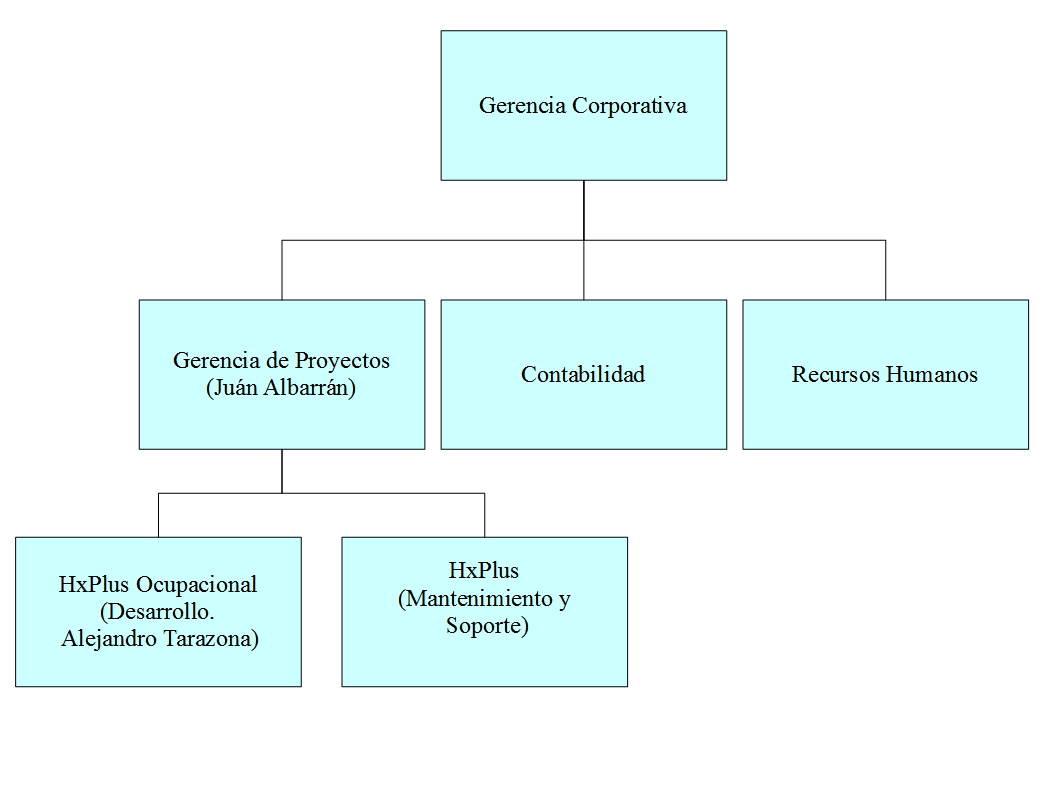
\includegraphics[scale=.25]{figures/Estructura}
        \end{center}
        \caption{Estructura Organizacional de Globinsoft}
        \label{estructura-org}
    \end{figure}

\pagebreak
     \chapter{Marco Teórico}

En el presente capítulo se describen conceptos y patrones utilizados para el desarrollo del proyecto de patantía, los cuales fueron seleccionados siguiendo los criterios de usabilidad, mantenibilidad, escalabilidad y portabilidad.

    \section{Modelo Vista Controlador (MVC)}
    
    El Modelo-Vista-Controlador es un patrón de arquitectura de \textit{software} que separa el modelo (Objetos de negocio) la vista (Interfaz con el usuario u otros sistemas) y el controlador (Manejo de la informacion de negocio)\cite{MVC-tiw}.
    
    Específicamente, cada componente tiene una asignación independiente de los demás componentes. Estas son:
    
    \begin{enumerate}
        \item \textbf{Modelo}
            \begin{itemize}
                \item Almacenamiento de los datos.
                \item Estado de la aplicación.
                \item Recuperación de errores en los datos.
            \end{itemize}
        \item \textbf{Vista}
            \begin{itemize}
                \item Presentación del modelo.
                \item Puede acceder al modelo pero no cambiar su estado.
            \end{itemize}
        \item \textbf{Controlador}
            \begin{itemize}
                \item Reaccionar a las peticiones del cliente.
                \item Comunicar al modelo de las acciones ejecutadas.
                \item Direccionar a las vistas requeridas del lado del cliente.
            \end{itemize}
    \end{enumerate}
    
    \section{Arquitectura Orientada a Servicios(SOA por sus siglas en inglés, \textit{Service Oriented Architecture})}
    
    A parte del patrón MVC que garantiza el bajo acoplamiento del sistema, se tiene la filosofía de desarrollo orientada a servicios la cual actúa como una guía de desarrollo y facilita el mismo orientado a la escalabilidad del sistema, esto es: facilita las actializaciones de alguno de los componentes MVC y minimiza el efecto que dicha actualización tiene sobre los demás.
    
    Según Gartner\cite{SOA-libroGartner} y González Quiroga\cite{SOA-tesis}, la incorporación de SOA empieza en las empresas hacia 2003, por las siguiente razones:
    
    \begin{itemize}
        \item La incesante presión de los negocios para la agilidad. Cuando una empresa quiere
        modificar sus procesos, productos o servicios, no puede permitirse el lujo de esperar por
        mucho tiempo. Debe ser posible cambiar la forma de aplicación de los sistemas de
        trabajo simplemente modificando los componentes que ya están en uso, en lugar de
        comprar o codificar nuevos componentes o sistemas enteros desde cero.
        
        \item La flexibilidad de la arquitectura SOA basada en Servicios Web de apoyo a múltiples
        aplicaciones.
        
        \item  La aceptación unánime de proveedores de los estándares de Servicios Web,
        especialmente de Simple Object Access Protocol (SOAP) y Web Service Description
        Language (WSDL)\cite{SOA-libroGartner}
        
    \end{itemize}
    
    SOA se basa en capas, cada una servicios a la siguiente y sus procedimientos internos se mantienen ocultos a las demás capas. Con esto se generan APIs de acceso estandarizado y son independientes de las tecnologías utilizadas en el desarrollo.
    
    En \textit{Service Oriented Architecture}\cite{SOA-msdn} definen SOA usando el poema de Saxe sobre los ciegos y el elfante.
    
    "Seis ciegos de Indostan se encuentran con un elefante, cada uno describe el elefante de forma diferente porque se ve influenciado por sus propias experiencias
    
    \begin{itemize}
        \item Quien le toca la trompa cree que es una serpiente.
        \item Quien le toca los colmillos cree que son lanzas.
        \item Quien le toca las orejas cree que son abanicos.
        \item Quien le toca la panza cree que es una pared.
        \item Quien le toca la cola cree que es una cuerda.
        \item Quien le toca	las patas cree que son árboles."
    \end{itemize}
    

    \begin{figure}
        \begin{center}
            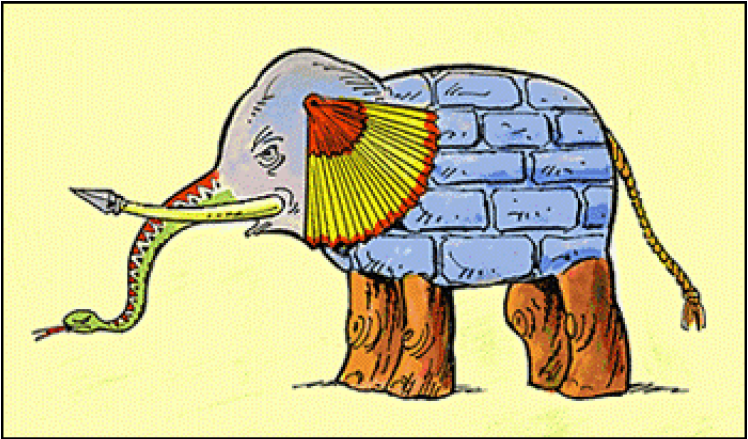
\includegraphics[scale=.75]{figures/Elefante}
        \end{center}
        \caption {El elefante de Saxe}
    \end{figure}

    Se usa la analogía para ejemplificar el hecho de que haya varias definiciones diferentes de lo que es SOA en si, porque se le ha definido como patrón de diseño o como una filosifía de desarrollo, siendo esta última la definición adoptada para el trabajo descrito en el presente informe.
    
    También se puede usar dicha analogía para ejemplificar cómo las (potenciamente) distintas vistas pueden interactuar con el controlador y este a su vez con el modelo.


    \section{Autenticación Basada en \textit{Tokens}}
    
    Es una forma de autenticación ligera\cite{ToTOKEN-tokenbasedauth}, que va de la mano con SOA, que usa \textit{tokens} o fichas cifradas para la verificación de usuarios. Estas fichas son almacenadas en el cliente y enviadas en cada una de los \textit{requests} que realiza el navegador, la ficha es decifrada y se verifican las credenciales del usuario en cuestión.
    
    Entre los datos almacenados en las fichas están:
    
    \begin{itemize}
        \item Nombre de usuario.
        \item Fecha de autenticación.
        \item Fecha de caducidad de la ficha.
    \end{itemize}
    
    Estas son cifradas en el servidor bajo una clave secreta elegida por el mismo servidor y que se usa para el posterior decifrado de las fichas.
    
    Todo esto permite que el servidor no se sobrecargue con variables de estado o de sesión por cada usuario autenticado en un momento dado y además permite la portabilidad desesada para el sistema.
    
\pagebreak
     \chapter{Marco Metodológico}

    En el presente capítulo se describe la metodología usada para el desarrollo del proyecto así como sus componentes, los actores que participaron y los roles que cumplieron en el desarrollo del mismo.

    Para \textit{HxPlus Ocupacional} fue seleccionado Scrum como metodología de desarrollo a seguir. Y aunque no está estipulado por la metodología, se llevaron a cabo diagramas de casos de uso y de clases para una documentación completa del sistema.
    
    Scrum es una metodología de gestión de proyectos ágil que utiliza uno o más equipos de trabajo, de a lo sumo 7 personas, en iteraciones de tiempo fijo, llamados \textit{Sprints}, para la entrega de tareas o avances en el proyecto que sean funcionales y probados
    \footnote{Con información de \citeauthor{scrum-guia}\cite{scrum-guia}, \citeauthor{scrum-primer}\cite{scrum-primer} y \citeauthor{scrum-agile}\cite{scrum-agile}}.    
    
    Los equipos apuntan siempre a conseguir avances limpios, probados y aceptados de manera que puedan ser puestos en producción inmediatamente.
    
    Scrum se divide en Roles, Eventos y Artefactos tal como se describe a continuación:

    \section{Roles}
        
        \subsection{Product Owner}
        \label{product-owner}
        
        Este rol representa la voz del cliente en la gestión del proyecto. Debe velar por la realización del proyecto desde la perspectiva del negocio. Se encarga de escribir las historias de usuario, las prioriza y las anexa al ``Product Balcklog" (o también Lista del Producto).
        
        El Dueño de Producto es la única persona responsable de gestionar la Lista del Producto. La gestión de dicha lista, según expresa \citeauthor{scrum-guia}\cite{scrum-guia}, consiste en:
        
        \begin{itemize}
            \item Expresar claramente los elementos de la Lista del Producto.
            \item Ordenar los elementos en la Lista del Producto para alcanzar los objetivos y misiones de la mejor manera posible.
            \item Optimizar el valor del trabajo desempeñado por el Equipo de Desarrollo.
            \item Asegurar que la Lista del Producto es visible, transparente y clara para todos, y que muestra aquello en lo que el equipo trabajará a continuación.
            \item Asegurar que el Equipo de Desarrollo entiende los elementos de la Lista del Producto al nivel necesario.
        \end{itemize}
               
        Para el presente proyecto se designó al ingeniero Juan Albarrán como Product Owner siendo el mejor representante de los intereses de Soluciones Globinsoft S.A. y estando él familiarizado tanto con los porcesos de negocio como con el equipo de desarrollo y el proceso de desarrollo mismo.
        
        \subsection{Scrum Master}
        \label{scrum-master}
        
        Es el responsable de llevar el procedimiento de gestión del proyecto según los lineamientos de Scrum. Sirve de asesoría entre invloucrados y comprometidos en materia de organización y distribución de la información. Él dirige las reuniones y vela por su cumplimiento según las reglas de procedimiento de Scrum.
        
        \citeauthor{scrum-guia}\cite{scrum-guia} clasifica los servicios del Scrum Master en tres categorías:
        \begin{enumerate}
            \item Servicio al dueño del producto
            \begin{itemize}
                \item Asesoramiento para la gestión eficiente de la Lista del Producto.
                \item Asesoramiento para la planificación del producto.
            \end{itemize}
            
            \item Servicio al equipo de desarrollo
            \begin{itemize}
                \item Apoyar en la organización del equipo.
                \item Eliminar los impedimientos y dificultades que limiten el progreso del equipo.
                \item Facilitar la organización de los eventos de Scrum según sea requerido.
                \item Guiar al equipo en entornos donde Scrum no haya sido del todo adoptado.
                \item Apoyar al equipo en dudas que surjan respecto a los eventos y artefactos de Scrum.
            \end{itemize}
            \item Servicio a la organización
            \begin{itemize}
                \item Liderar la adopción de Scrum como metodología de desarrollo.
                \item Asesorar a los empleados en el uso de Scrum y sus procedimientos.
            \end{itemize}
        \end{enumerate}
        
       Por su experiencia en previos proyectos, entre ellos \textit{HxPlus} (antecedente de \textit{HxPlus Ocupacional}) y su amplio conocimiento en el negocio, se le delegó también el puesto de ``Scrum Master" en el presente proyecto al ingeniero Juan Albarrán.
        
        \subsection{Development Team}
        \label{development-team}
        
        Es el conjunto de personas dedicadas a construir el producto indicado por el dueño del producto. Se requieren que sean grupos lo suficientemente pequeños como para fomentar un alto nivel de independencia y autoorganización pero, a su vez, lo suficientemente grandes como para poder presentar avances significativos en cada Sprint y que potencialmente, estos avances, puedan ser puestos en producción.
        
        Equipos pequeños, de menos de tres personas, reduce la productividad global y reduce los posibles avances en el producto. También podrían presentar limitaciones en cuando a las habilidades de los integrantes, lo cual resultaría convirtiéndose en impedimentos en el desarrollo.
        
        Por otro lado, equipos muy grandes, de más de nueve miembros requiere demasiada coordinación entre los miembros lo cual podría significar una menor eficiciencia y mayor trabajo para la organización de los avances. En otras palabras, se perdería agilidad tratando de organizar un equipo semejante.
        
        Idealmente un equipo de desarrollo varía entre tres y siete personas. Esto mantiene un equilibrio saludable entre la cantidad de trabajo que pueden manejar y la capacidad de autoorganización del equipo.
        
        El equipo debe ser multifuncional, debe tener las capacidades necesarias para desarrollar el producto y poder apoyarse entre sí para compensar los puntos débiles de cada individuo.
        
        No existen roles dentro del equipo de desarrollo. A pesar que uno podría desempeñarse mejor en un área de desarrollo, no existen como tal roles. Esto es debido a que la responsabilidad del desarrollo recae sobre el equipo como un todo y sobre ningún miembro en particular, por ello tampoco existe un rol de Líder o Jefe de Proyecto.
        
        Para HxPlus Ocupacional el equipo de desarrollo consta de un solo miembro, Alejandro Tarazona, pasante y autor del presente libro.
        
    \section{Eventos}
    
    Esta sección describe los eventos determinados por la metodología seleccionada y cómo fueron establecidos para la gestión del proyecto. Estos son:
    
    \begin{figure}[htbp!]
        \begin{center}
            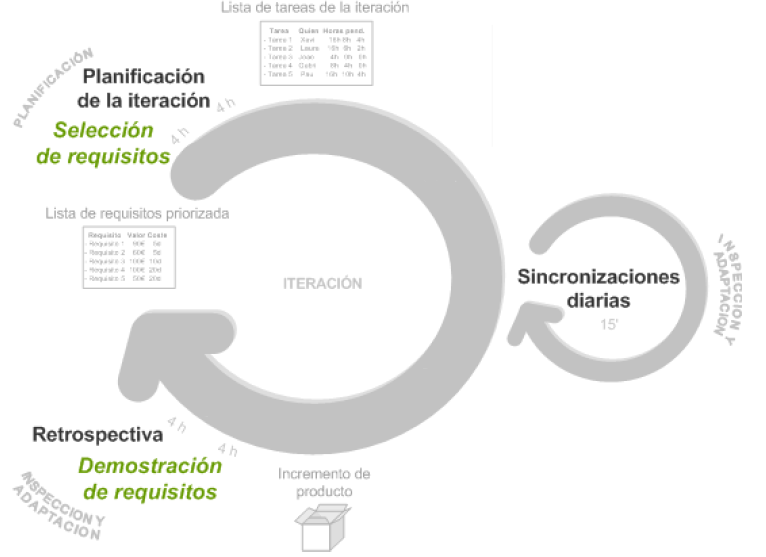
\includegraphics[width=.8\textwidth]{figures/scrum}
        \end{center}
        \caption{Esquema de trabajo de SCRUM}
        \label{scrum-esquema}
    \end{figure}
    
        \subsection{Sprint}
        
        Unidad mínima de desarrollo, usualmente determinada por una tarea corta o un período de tiempo pequeño, usualmente 1 o 2 semanas, nunca más de 30 días; durante el cual el equipo de desarrollo trabaja según las metas estipuladas al principio del mismo. Normalmente éstas metas no cambian durante el desarrollo del Sprint sino al final del mismo, cuando se planifica el siguiente Sprint.
        
        Para HxPlus Ocupacional fue determinado en una semana para las primeras tareas y dos para las últimas, debido a las pruebas subyacentes y el trabajo de integración que representan.
        
        Se llevaron a cabo 3 fases:
        \begin{enumerate}
            \item Preparación (1 Sprint)
            \item Desarrollo (8 Sprints)
            \item Cierre (2 Sprint)
        \end{enumerate}
        
        Tal y como se describe en el capítulo \ref{desarrollo-capitulo}.
        
        \subsection{Sprint Planning}
        
        Planificación del siguiente Sprint a realizar. El equipo de desarrollo (``Development Team", punto \ref{development-team}) hace los pronósticos e indica qué puede llevar a cabo en el siguiente Sprint de lo que propone el dueño del producto (``Product Owner", punto \ref{product-owner}) que debe hacerse durante el Sprint. El ``Scrum Master" (punto \ref{scrum-master}) está encargado de revisar cuidadosamente con el equipo las posibilidades, negociar con el dueño del producto las posibilidades de realización y establecer las metas.
        
        Semanalmente se realizó una reunión del \textit{Development Team} con el \textit{Scrum Master} y \textit{Product Owner} para evaluar el resultado del Sprint de esa semana y realizar la planificación adecuada a los logros y el desenvolvimiento en el proyecto.
        
        \subsection{Daily Sprint Meeting}
        
        Reuniones diarias realizadas entre el ``Scrum Master" y el equipo de desarrollo para revisar los avances diarios, aclarar dudas y difundir información acerca del progreso alcanzado hasta el momento. Tiempo fijo en 15 minutos y usualmente se realizan en la mañana.
        
        En este punto, Scrum, hace una diferenciación clave entre los elementos que están compromentidos (\textit{``commited"}) y los que sólo están involucrados (\textit{``involved"}) en el desarrollo del proyecto. Siendo comprometidos los equipos de desarrollo, el ``Scrum Master" y el ``Product Owner" e involucrados los demás departamentos de la empresa que puedan tener interés en el estado del proyecto (dpto. de ventas, clientes, etc). 
        
        En este órden de ideas, durante una reunión diaria de Sprint, sólo los comprometidos tienen potestad de hablar o comentar las cosas que han sucedido. Esto se hace para lograr que, en los 15 minutos de duración de la reunión, se discutan temas que sean de suma necesidad para el desarrollo del proyecto, se ponen de manifiesto dificultades técnicas o impedimentos dentro de los equipos de desarollo y, también, para difundir información sobre el estado del proyecto a las partes involucradas.
        
        La responsabilidad de resolver todo impedimento manifestado en dichas reuniones recae sobre el ``Scrum Master".
        
        Durante el proyecto se realizaron las reuniones con la presencia del Ing. Juan Jesús Albarrán para actualizar el estado del desarrollo del proyecto y aclaración de dudas por parte del pasante en cuanto a lo acaecido durante el día previo.
        
        \subsection{Sprint Review}
        
        Son reuniones que se realizan, como su nombre lo indica, para hacer una revisión del trabajo realizado durante el Sprint y presentar el trabajo completado a las partes involucradas. Estas reuniones no deben pasar de 4 horas de duración y todo trabajo incompleto no debe ser presentado.
        
        Una vez mostrados los resultados del Sprint, el ``Product Owner" debe realizar una evaluación de las metas cumplidas (o no) y si ha habido cambios en el contexto, deberá también realizar las adaptaciones necesarias a la planificación del proyecto.
        
        En \textit{HxPlus Ocupacional} se realizaoron en conjunto las reuniones de \textit{Sprint Planning} y \textit{Sprint Review} del último Sprint finalizado con la finalidad de minimizar el tiempo de reuniones y aprovechar las disponibilidades de los comprometidos y los involucrados.
        
        \subsection{Sprint Retrospective}
        
        Al finalizar cada Sprint el equipo se reúne con un tiempo fijo de 4 horas para revisar sus técnicas y la forma en que han abordado el desarrollo del proyecto, discutir las impresiones referentes al Sprint superado y revisar los inconvenientes presentados.
        
        Es deber del ``Scrum Manager" revisar los inconvenientes y buscarles solución rápida para mejorar la productividad del equipo.
        
        Debido al que el grupo de trabajo sólo consta de 1 desarrollador, se consideró inconveniente realizar reuniones de 4 horas exclusivamente para hacer la restrospectiva. En su lugar se atendieron los inconvenientes, dudas y revisones durante las reuniones diarias y se apartó un espacio de 15 minutos de las reuniones de planificación y revisión para realizar actividades de ésta reunión.
        
    \section{Artefactos}
    
    Documentos realizados para llevar registro de las etapas de desarrollo del proyecto y a su vez realizar la evaluación de las mismas.
    
        \subsection{Product Backlog}
        
        O también ``Lista de Producto". Es una lista con todas las consideraciones necesarias de parte del dueño del producto, quien la organiza y la gestiona. Cualquier cambio a realizarse dentro de la planificación debe pasar por esta lista.
        
        En esta lista se enumeran los deseos del cliente, se priorizan y se estima el esfuerzo requerido. Esta lista debe ser seguida por el equipo de desarrollo para dirigir sus avances.
        
        Es una lista que hace el Dueño del Pruducto iniciando el proceso de gestión de requerimientos, sin embargo, esta lista tiene la característica de ser mutable, como los requerimientos del Dueño del Producto, y es modificada conforme sea necesario o requerido. Por eso es que \citeauthor{scrum-guia}\cite{scrum-guia} dice: ``Una Lista de Producto nunca está completa".
        
        Para ello existe el ``refinamiento" de la lista del  producto, el cual  es el proceso de añadir detalles, granularidad y prioridad a cada uno de los requerimientos, según \citeauthor{scrum-guia}\cite{scrum-guia}. Usualmente, las tareas o requerimientos que pasan a ser parte de la siguiente planificación de Sprint son las de mayor prioridad y granularidad y que, además, suele ser el caso que las actividades prioritarias son refinadas primero para así llevarlas a desarrollo lo antes posible.
        
        En el caso de \textit{HxPlus Ocupacional} el Dueño del producto realizó un levantamiento de requerimientos y utilizó ``Trello" para la gestión de los requerimientos.
    
        \subsection{Sprint Backlog}
        
        O ``Lista de Pendientes del Sprint". Es una lista de objetivos del Sprint tomada de la lista de producto durante la planificación del Sprint. Puede ser uno o varios objetivos, lo suficientemente refinados como para que el equipo de desarrollo pueda entenderlos en la reunión diaria y puedan ser llevados a cabo durante el Sprint.
        
        Según se requiera nuevo trabajo, el equipo de desarrollo lo irá añadiendo a la lista de pendientes del Sprint, ya sea por inconvenientes surgidos o problemas no tomados en cuenta o por refinamiento de los objetivos. Además, conforme el trabajo vaya siendo completado, se debe actualizar la estimación del trabajo restante. Sólo el equipo de desarrollo tiene potestad sobre la lista de pendientes del Sprint y es su forma de ver, transparentemente y en tiempo real, el estado del dearrollo de un Sprint.
        
        Usando también las facilidades de ``Trello", el equipo de desarrollo gestionó cada Sprint a través de las listas creadas dentro de una ``Pizarra" del sistema.
    
\pagebreak
     \chapter{Marco Tecnológico}

En este capítulo se presentarán las herramientas y protocolos utilizados durante el desarrollo del proyecto, ya sea para el desarrollo en sí mismo o para el apoyo en cuanto a control de versiones y gestión de tareas.

    \section{Herramientas para el desarrollo de la aplicación}
    
    En esta sección se describen las herramientas usadas en el desarrollo de la aplicación y las características que hicieron que fueran seleccionadas para tal fin.
    
        \subsection{Eclipse}
        \label{tecno-eclipse}
        
        Es un entorno integrado de desarrollo (IDE) basado en Java. Provee las librerías necesarias para el desarrollo, facilita la configuración del proyecto y hace uso de herramientas como Maven para la gestión de librerías del proyecto.
        
        Combina un compilador junto con facilidades para la configuración de diferentes servidores, tanto de bases de datos como servidores web para atender los servicios del \textit{back end}.
        
        Usando esta herramienta se procedió a la configuración de los repositorios de Maven (ver \ref{tecno-maven}), el servidor tomcat (ver \ref{tecno-tomcat}), el entorno de desarrollo de Java y su respectivo entorno de ejecución (ver \ref{tecno-java}).
        
        En el desarrollo de ``HxPlus Ocupacional" se utilizó \textit{Eclipse Kepler} en su versión de 64 bits para Linux - Debian 9.
        
        \subsection{apache}
        \label{tecno-apache}
        
        Es un servidor web multiplataforma. Utiliza el protocolo http para la transferencia de información con los clientes y posee soporte de seguridad para SSLy TLS\cite{APACHE-culturacion}. Posee licencia GPL y una comunidad de desarrolladores que mantiene el servidor actualizado continuamente.
        
        Dadas sus características \textit{open source} se cuenta con equipos de desarrolladores alrededor del mundo que además funjen como soporte del mismo, lo cual lo hace un servidor altamente utilizado y con muy buena capacidad de respuesta en caso de inconvenientes con el mismo.
        
        Está alojado dentro del servidor de ``Apache Foundation"\cite{APACHE-maven} en donde además se alojan otras herramientas utilizadas en el proyecto.
        
        Para ``HxPlus Ocupacional" se designó Apache como servidor web exclusivo de \textit{front end}. Se hace incapié en ello ya que dada la orientación a servicios del sistema, se pueden crear nuevos servidores, para dispositivos móbiles primordialmente, que están dedicados exclusivamente a su función y no cambiarían la forma de interacción de este servidor.
        
        \subsection{Tomcat}
        \label{tecno-tomcat}
        
        Apache Tomcat, 	Jakarta Tomcat o comunmente llamado Tomcat es un servidor web especializado en el almacenamiento de sistemas web bajo las especificaciones JSP (JavaServer Pages) de Oracle Corporation, aunque fue creado, originalmente, por Sun Microsystems.
        
        Siendo parte de Apache Foundation, también posee licencia GPL y es de código abierto, con una comunidad que desarrolla, bajo ``Java Comunity Process", las especificaciones de Java Servlet, JavaServer Pages, Java Expression Language y Java WebSocket\cite{APACHE-tomcat}.
        
        Este servidor fue instalado y configurado para hospedar el \textit{back end} de ``HxPlus Ocupacional" y los servicios que ofrece. Tomando la filosofía de SOA (Ver \ref{teorico-soa}), en este servidor estarán alojados los servicios que proporcionará el sistema, para ser usados por las distintas implementaciones del \textit{front en}.
    
        \subsection{Java}
        \label{tecno-java}
        
        Lenguaje de programación utilizado para el desarrollo del \textit{backend}. Java es un lenguaje de programación imperativo orientado a objetos que facilita el desarrollo independiente de los servicios y el fácil acceso al modelo de datos permitiendo así la baja cohesión entre los componentes del sistema.
        
        El entorno de desarrollo (JDK) y de ejecución (JRE) fue Java 8. Ya que porvee las últimas actualizaciones de las librerías de Java y previene problemas de seguridad por puertas traseras presentados en la versión 7. Además que ofrece facilidades adicionales en lo que se refiere a la utilización de herramientas como Hibernate, JPA e iText.
        
        \subsection{JSON}
        \label{tecno-json}
        
        Por \textit{JavaScript Object Notation}, es un formato de intercambio de datos, ligero\cite{JSON-yahoo} que permite una sencilla comunicación entre la vista y el controlador. También permite la fácil depuración y la visualización de los datos enviados, dentro del entorno de desarrollo, para la verificación y corrección de errores.
        
        JSON es un formato de texto que es independiente del lenguaje. Utiliza convenciones que son  conocidos por los programadores de Java, JavaScript, Perl, Python, y otros. Estas propiedades hacen que JSON sea el lenguaje ideal para el intercambio de datos\cite{JSON-jsonOrg}.
        
        JSON se contruye de la siguiente forma:
        
        \begin{itemize}
            \item Todo objeto atómico comienza y termina con ``\{\}" (llaves).
            \item Los objetos llevan nombre del objeto seguido de ``:" y el valor del objeto.
            \item Si el valor del objeto es compuesto (varios atributos), los componentes se enlistan entre llaves y separados por ``," (coma).
            \item Los atributos de un objeto son siempre un par \textit{nombre:valor}. Siendo ``nombre" el nombre del atributo. Es similar a la sintaxis usada para el nombre del objeto.
            \item Listas o arreglos de objetos son nombrados como un objeto atómico mas una ``s" al final del nombre.
            \item Los arreglos van enmarcados de ``[]" (corchetes).
        \end{itemize}
        
        \begin{figure}[htbp!]
            \begin{center}
                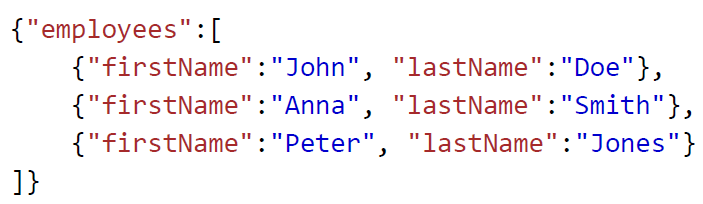
\includegraphics[width=.8\textwidth]{figures/jsonejemplo}
            \end{center}
            \caption{Ejemplo de lista de empleados genérica en \textit{JSON}}
            \label{json-ejemplo}
        \end{figure}
        
        Fue elegido por su compatibilidad con Java y porque es independiente de la tecnología usada en la vista, lo cual permite a su vez realizar cambios en la vista sin afectar las funcionalidades del controlador.
        
        \subsection{JPA}
        \label{tecno-jpa}
        
        Por ``Java Persistence API", proporciona un modelo de persistencia basado en objetos de Java planos (POJO, por sus siglas en inglés \textit{Plain Old Java Object}) para hacer la correspondencia con las entidades en la base de datos\cite{JPA-definicion}. En la práctica, hace transparentes las consultas y acciones realizadas sobre la base de datos.
        
        Como tal, JPA, no implementa los modelos de persistencia que usará la base de datos si no que proporciona un estándar para que se puedan mantener las caractarísticas de la orientación a objetos de Java y se puedan enlazar, uno a uno, con las entidades, atributos y relaciones de la base de datos.
        
        JPA se puede configurar vía anotaciones o usando un documento XML que debe ser distribuido junto con el sistema. En el caso de ``HxPlus Ocupacional" se eligió la configuración por anotaciones debido que está presente directamente en los objetos (clases) de Java y permite una mejor mantinibilidad del código.
        
        Entre las implementaciones conocidas de JPA tenemos:
        \begin{itemize}
             \item Hibernate
             \item ObjectDB
             \item EclipseLink
             \item OpenJPA
        \end{itemize}
        
        Siendo la implementación de Hibernate la seleccionada por lo descrito en el punto \ref{tecno-hibernate}.
        
        \subsection{Angular JS}
        \label{tecno-angular}
        
        Es un \textit{framework}orientada a facilitar el desarrollo web de aplicaciones dinámicas del lado del cilente. ``AngularJS le permite extender el vocabulario HTML para su aplicación"\cite{ANGULARJS-angularjs}. Utiliza lo que llama ``directivas" que son bloques de código en javascript que ayudan a estructurar las acciones del \textit{front-end}. También maneja ``atributos" y ``elementos" que pueden ser programados separadamente del código HTML y luego insertados en dicho archivo para su utilización.
        
        Provee asociación birireccional de variables del DOM lo cual simplifica drásticamente las pruebas del lado del cliente y mantiene, como se mencionó anteriormente, la estructura organizada del código. La asociación bidireccional a través de ``expresiones" se utiliza para mantener actualizado al cliente en cuanto a cambios que se realizen en las variables internas y mejora la respuesta visual sin realizar una recarga de la página.
        
        El código de Javascript (punto \ref{tecno-javascript}) debe ser importado en el archivo HTML en que se quieren utilizar. Existen dos formas de importarlas, desde el servidor de google\footnote{http://ajax.googleapis.com/ajax/libs/angularjs/1.4.8/angular.min.js} o descargando los archivos al servidor local y agregando la dirección local.
        
        Por todo esto, se eligió AngularJS para su utilización como \textit{framework} del \textit{front end} del sistema.
        
        \subsection{JavaScript}
        \label{tecno-javascript}
        
        JavaScript es un lenguaje de programación interpretado, dialecto del estándar ECMAScript. Se define como orientado a objetos, basado en prototipos, imperativo, débilmente tipado y dinámico\cites{JAVASCRIPT-wiki}{JAVASCRIPT-manual}. También posee soporte en casi todos los navegadores utilizados actualmente.
        
        Es un lenguaje de programación orientado a crear contenidos dinámicos para páginas web del lado del cliente. AngularJS, previamente mencionado, usa JavaScript como lenguaje de programación para su implementación.
        
        \subsection{MySQL}
        \label{tecno-mysql}
        
        Manejador de bases de datos, posee licencia GPL y licencia comercial de Oracle\cite{MYSQL-referencemanual}. Ofrece alto rendimiento, eficiencia y seguridad en el almacenamiento y recuperación de datos\cite{MYSQL-oracle}. Comúnmente utilizado en entornos de desarrollo LAMP para desarrollo web.
        
        Es un manejador multi-hilo, multi-usuario y robusto, está diseñado para soportar altos niveles de carga y ser utilizado en entornos de producción con fuerte afluencia de datos. Además de poseer librerías ampliamente usadas para Java las cuales ayudan al desarrollo debilmente acoplado del \textit{back-end}.
        
        Para ``HxPlus Ocupacional" se eliegió este manejador, haciendo uso de su licencia GPL, para el desarrollo del sistema.
        
        \subsection{SPRING}
        \label{tecno-spring}
        
        Framework para el desarrollo de aplicaciones que provee inversión de control; es de código abierto y está diseñado sobre Java. Permite integración con Hibernate, JPA y JSON\cite{SPRING-essential}.
        
        SPRING fue diseñado para facilitar el desacoplamiento de los compomentes del sistema utilizanco IOC. Esto permite que los componentes sean desarrollados una y sólo una vez y que puedan ser reutilizados en diferentes contextos\cite{SPRING-referencedoc}.
        
        Su fácil integración con Hibernate y, por consecuencia, con JPA permite que la interacción con la base de datos sea transparente al desarrollador y evita que tenga que reescribirse el código en caso de cambios en el manejador (de bases de datos) utilizados.
        
        
        \subsection{Maven}
        \label{tecno-maven}
        
        Es una herramienta de gestión y manejo de librerías, parecida a ``Apache Ant". Utiliza el concepto del ``Modelo del Objeto de Proyecto" (del inglés \textit{Project Object Model}, o POM) para gestiónar la construcción del proyecto dónde se utilice. Esto es, gestiona las librerías, dependencias y versiones (de las librerías) de forma centralizada y limpia.
        
        El POM es un archivo en formato XML dónde se registran las librerías que serán usadas por el proyecto  para que el manejador de Maven se encargue de la descarga de las mismas. Se gestiona a través de artefactos que registran la información de una librería de acuerdo con la figura \ref{pom-artifact}.
        
        \begin{figure}[htbp!]
            \begin{center}
                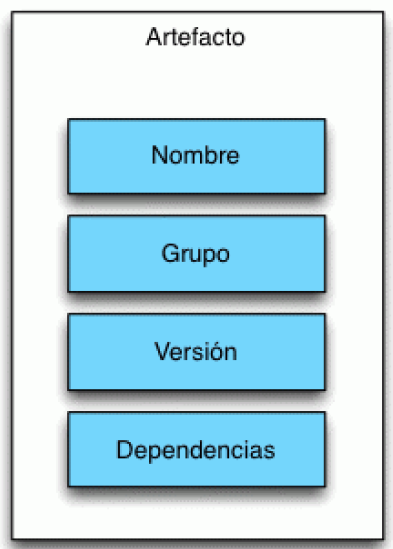
\includegraphics[scale=0.4]{figures/pomartifact}
            \end{center}
            \caption{Artefacto de Maven y descripción de su contenido.}
            \label{pom-artifact}
        \end{figure}
        
        La estructura del POM puede llegar a ser tan compleja como el proyecto que gestiona, llegando incluso a depender de otros POM. En ``HxPlus Ocupacional" se manejó usando un sólo POM de la manera más sencilla posible.
        
        En \citetitle{APACHE-maven}\cite{APACHE-maven} mantienen repositorios de librerías actualizados y correctamente asociados a las dependencias de dichas librerías.
        
        \subsection{Hibernate}
        \label{tecno-hibernate}
        
        Es un framework de persistencia que provee una implementación de JPA\cite{HIBERNATE-basico}. Gestiona las comunicaciones a nivel de nombres de entidades y atributos con su respectiva contraparte de Java, clases con sus atributos. A esto se le conoce como ``Correlación Objeto-Relacional" (ORM, por su siglas en inglés \textit{Object Relational Mapping}).
        
        Esta correlación que crea Hibernate permite ciertas facilidades al momento de manejar las distintas interacciones con la base de datos que devienen en un código mantenible en el tiempo.
        
        El framework es integrado al desarrollo a través de Maven y tiene soporte para los siguientes manejadores de bases de datos\cite{HIBERNATE-tutorial}: 
        \begin{itemize}
            \item MySQL
            \item PostgreSQL
            \item Oracle
            \item DB2/NT
            \item HSQL Database Engine
            \item entre otros...
        \end{itemize}
        
        Tradicionalmente se utilizan dos archivos de configuración (llamados ``hibernate.properties" y ``hibernate.cgf.xml") que se modifican con cada nueva tabla o ``clase de persistencia" que se requiera, sin embargo este método tiende a no ser mantenible en el tiempo ya que debe buscarse dentro de estos archivos las configuraciones de las clases y no existe un orden estipulado para la creación y modificación de estos archivos. Para evitar esto, y dado que se tiene una versión de Java opsterior a JDK 5, se procedió a la utilización de la versión 3 de hibernate que incorpora librerías para el uso de anotaciones, quedando así la configuración de las clases de persistencia dentro del código de las clases de Java, lo cual permite y permitió, durante el desarrollo, fácil depuración de errores y un sencillo mantenimiento del código.
        
        \subsection{iText}
        \label{tecno-itext}
        
        Herramienta de generación de PDF dinámicos\cite{ITEXT-basico}. Proporciona un API que permite la generación de archivos PDF usando la información enviada.
        
        Actualmente existen módulos de gestión, interpretación y conversión de archivos PDF, sin embargo para efectos de ``HxPlus Ocupacional" sólo se utilizó el módulo de generación de los mismos.
        
        Su integración con Maven permitió la fácil descarga de la librería y su configuración dentro del proyecto. Para su uso sólo se necesitó la creación de una clase dentro del \textit{back end}, que contiene las importaciones requeridas para así poder generar los PDF necesarios.
        
    \section{Herramientas para el control de versiones y planificación}
    
    En la presente sección se presentan las herramientas de planificación y control de versiones usadas durante el desarrollo de la aplicación. Si bien no están vinculadas directamente al código, las mismas sirvieron de soporte para la organización del proyecto.
    
        \subsection{Git}
        \label{tecno-git}
        
        Es un sistema de control de versiones distribuido, diseñado por Linus Torvalds, enfocado en eficiencia, integridad de datos, velocidad de transferencia y soporte para flujos de trabajo no lineales.
        
        Siguiendo este enfoque, se logró un \textit{software} que almacena los archivos relativos a un proyecto tomando como base un directorio ``raiz" y los archivos y directorios que lo conformen, incluye recursivamente los archivos y directorios dentro del directorio raiz, y  a partir de ellos almacena los cambios realizados a la última versión, sin modificar los archivos originales ni los archivos de modificaciones; con ello se logra que los cambios puedan ser reversibles y que sean almacenados con poco uso de memoria, reduce la carga de datos al momento de crear repositorios remotos ya que no se está enviando los archivos completos sino los archivos de cambios.
        
        Para el caso de repositorios remotos y el manejo de la carga, también incluye la restricción de versiones. Un usuario debe tener en el repositorio local la última versión disponible, en caso de que la última versión esté en el repositorio local, se cargan los cambios normalmente al repositorio remoto; en caso contrario, el usuario debe descargar la última versión del repositorio remoto, (potencialmente) resolver conflictos que puedan surgir entre los archivos modificados de manera local y los que hayan sido modificados en el servidor remoto y luego hacer la carga al servidor remoto.
        
        También ofrece la posibilidad de crear ``ramas" de desarrollo. Esto es, cambios y modificaciones de un proyecto que parten de una raiz pero que puede tener una meta diferente. Esto facilita el proceso cuando existen varios desarrolladores trabajando en paralelo sobre el mismo proyecto, aunque en el caso de surgir conflictos en los cambios puede llegar a ser engorrosa la integración (\textit{merge}) del código.
        
        Para HxPlus se crearon dos repositorios raices, dadas implicaciones de permisos de ejecución dentro del sistema operativo elegido. Estos repositorios fueron llamasdos ``occupational" y ``proyectoAngular" refiriendose al \textit{back-end} y \textit{front-end} respectivamente.
        
        \subsection{GitHub}
        \label{tecno-github}
        
        Servidores online de repositorios remotos para Git. Puede ser usado de manera gratuita y pública. Permite el acceso a los repositorios de manera ininterrumpida y global.
        
        Los repositorios fueron almacenados en la cuenta personal de Alejandro Tarazona, en el url: \textit{http://www.github.com/atarazona89} con los nombres descritos con anterioridad, para su almacenamiento en la web.
        
        \subsection{Trello}
        \label{tecno-trello}
        
        Herramienta diseñada con la misión de facilitar la gestión de tareas usando listas o tablas. Cuenta con una interfaz intuitiva y de fácil aprendizaje para llevar a cabo dicha misión. Una vez creadas las tablas que se desean, se pueden crear tareas dentro de ellas, las cuales a su vez pueden ser etiquetadas, organizadas o comentadas por los participantes. Las tareas pueden ser arrastradas entre las listas emulando así la transición entre los estados de desarrollo del proyecto.
    
\pagebreak
     \chapter{Desarrollo de la Aplicación}
\label{desarrollo-capitulo}

En el presente capítulo se presenta, de forma detallada, cómo fue el desarrollo del proyecto, los objetivos y actividades específicas de cada \textit{Sprint} y finaliza con una revisión de dificultades técnicas y los resultados del proyecto.

\section{Fase de Preparación}
    \subsection{Primer Sprint}
    
    En este \textit{sprint} se realizó las descargas de herramientas y la creación de los diagramas que serán la guía de desarrollo del sistema.
    
    \begin{enumerate}
        \item Objetivos
        \begin{enumerate}
            \item Levantar los requerimientos del producto.
            \item Documentación de la aplicación.
            \item Introducción al ambiente de trabajo.
        \end{enumerate}
        \item Actividades
        \begin{itemize}
            \item Creación del \textit{Product Backlog}
            \item Documentar la aplicación.
            \item Creación del diagrama ER-E para la base de datos de la aplicación.
            \item Creación de un modelo de casos de uso de la aplicación.
            \item Descarga de las herramientas ya mencionadas en el marco tecnológico.
        \end{itemize}
    \end{enumerate}
        
\section{Fase de Desarrollo}
    
    \subsection{Primer Sprint: Configuración de la aplicación}
    
    En este \textit{sprint} se configuraron Eclipse, Apache y MySQL para crear un ambiente de desarrollo adecuado para el sistema a desarrollar.
    
    \begin{enumerate}
        \item Objetivos
        \begin{enumerate}
            \item Crear y configurar el ambiente de desarrollo
            \item Descargar y configurar las herramientas necesarias para el desarrollo
            \item Descargar y configurar las herramientas necesarias para la gestión del proyecto         
        \end{enumerate}
        \item Actividades
        \begin{itemize}
            \item Creación de cuenta y tablas en Trello para la gestión del proyecto
            
            Las tablas de notas usadas fueron ``Pendiente", ``Impedido", ``En desarrollo" y ``Tarminado"; para referirse al estado actual de las tareas en cada una de las listas.
            
            \item Creación de repositorios
            
            Se crearon los repositorios Git tanto local como remoto, para el almacenamiento de la aplicación usando Git y Github como sitio de almacenamiento para los repositorios remotos. Los repositorios están bajo los nombres de ``ocupacional" y ``proyectoAngular" en el url: \textit{www.github.com/atarazona89}.
            
            \item Diseño de la Base de Datos
            
            Creación del diagrama ER-E y el glosario de términos de la aplicación. Ver apéndice \ref{ere}.
            
            \item Descarga del \textit{IDE} Eclipse
            
            Para el desarrollo se utilizo Eclipse Kepler, descargado de la página oficial de Eclipse\cite{ECLIPSE-eclipseorg}
            
           \item Descargar y configurar \textit{plugins} de Eclipse
           
           Se realizaron los cambios necesarios en la configuración del ``pom.xml" para así acceder a los repositorios de Maven que contienen las distintas librerías tanto de SPRING como de las distintas herramientas ya mencionadas. Se realizó la depuración de los archivos y la respectiva configuración adecuada al ambiente de trabajo. Esto se refiere a la configurar Eclipse para usar \textit{SPRING} como \textit{framework}, Hibernate y Liquibase como gestores de comunicación con la base de datos y configurar la base de datos con las credenciales de MySQL asignadas para el desarrollo del proyecto.
           
           \begin{table}[h!]
               
               \begin{center}
                   \begin{tabular}{|l|l|l|}\hline
                       Grupo & Artefacto & Versión \\\hline
                       org.springframework & spring-core & 4.1.2.RELEASE \\\hline
                       org.springframework & spring-orm & 4.1.2.RELEASE \\\hline
                       org.springframework & spring-webmvc & 4.1.2.RELEASE \\\hline
                       mysql & mysql-connector-java & 5.1.9 \\\hline
                       org.liquibase & liquibase-plugin & 1.6.1.0 \\\hline
                    \end{tabular}
                \end{center}
                
                \caption{Artefactos de Maven: Spring}
                \label{artefactos-spring}
           \end{table}
            
           Aunque, en lo referente a liquibase, se utilizó un plugin, no una librería. Ver cuadro \ref{artefactos-hibernate}.
           
           \item Configuración de las características de \textit{SPRING} para trabajar con anotaciones
           
           Se realizaron los cambios dentro del archivo ``occupational-servlet.xml" que permiten el uso de anotaciones para el direccio amiento interno de los procesos.
           
           
           \item Descargar y configurar la librería de JSON para la comunicación con el \textit{front-end}
           
           Usando los repositorios de Maven se descargaron las librerías necesarias de JSON para la comunicación. Las dependencias descargadas fueron, del grupo \textit{com.fasterxml.jackson.core}, las enumeradas en el cuadro \ref{artefactos-json}.
           
           \begin{table}[h!]
               
               \begin{center}
                    \begin{tabular}{|l|l|}\hline
                       Artefacto & Versión \\\hline
                       jackson-core & 2.2.2 \\\hline
                       jackson-annotations & 2.2.2 \\\hline
                       jackson-databind & 2.2.2 \\\hline                   
                    \end{tabular}
                \end{center}
                
                \caption{Artefactos de Maven: JSON}
                \label{artefactos-json}
            \end{table}
           
           \item Descargar y configurar las librerías de Hibernate para la comunicación con la base de datos
           
           Usando Maven fueron descargadas las librerías de Hibernate que usan JPA como API para comunicarse con la base de datos.
           
           \begin{table}[h!]
               
               \begin{center}
                   \begin{tabular}{|l|l|l|}\hline
                       Grupo & Artefacto & Versión \\\hline
                       org.hibernate.javax.persistence & hibernate-jpa-2.0-api & 1.0.1.Final \\\hline
                       org.hibernate.common & hibernate-commons-annotations & 4.0.4.Final \\\hline
                       javax.persistence & persistence-api & 1.0.2 \\\hline
                       org.hibernate & hibernate-entitymanager & 4.1.9.Final \\\hline
                       org.springframework.data & spring-data-jpa & 1.8.1.RELEASE \\\hline
                    \end{tabular}
                \end{center}
                
                \caption{Artefactos de Maven: Hibernate}
                \label{artefactos-hibernate}
            \end{table}
           
        \end{itemize}
    \end{enumerate}
        
        
    \subsection{Segundo Sprint: Configuración de la aplicación}
    
    En este \textit{sprint} se relizaron las configuraciones necesarias de las herramientas y la creación de funcionalidades básicas del lado del servidor para empezar el desarrollo del sistema.
    
    \begin{enumerate}
        \item Objetivos
        \begin{enumerate}
            \item Creación de clases, repositorios y servicios básicos.
            \item Creación de controladores básicos.
        \end{enumerate}
        \item Actividades
        \begin{itemize}
            \item Crear las siguientes clases para manejo de la información:
            \begin{itemize}
                \item Usuario
                \item Paciente
                \item Doctor
                \item Empresa
                \item Centro de Costos
                \item Sede
                \item Departamento
                \item Consulta
                \item Nota de revisión (\textit{SoapNote}, por \textit{Subjective, Objective, Assessment, Plan})
                \item Diagnóstico
                \item Examen
                \item Consulta
                \item Récipe
                \item Medicamento
                \item Laboratorio
            \end{itemize}
            
            \item Crear los repositorios
            
            En este entorno `repositorios' se refiere a las interfaces que usa \textit{Hibernate} para manejar los accesos y consultas con la base de datos. Estos repositorios vienen con métodos y procedimientos  implemantados por Hibernate y estipulados por JPA.
            
            Se creó un paquete de clases, llamado ``repositories", con un repositorio para cada una de las clases mencionadas anteriormente.
             
            \item Crear los servicios para las clases
            
            Los servicios están compuestos por una interfaz y su respectiva implementación por cada una de las clases mencionadas. Estos servicios se encargan de procesar la información haciendo uso de los repositorios, en caso de ser necesario, para brindar respuestas encapsuladas a los respectivos controladores.
            
            \item Crear los controladores de la aplicación
            
            En este \textit{Sprint} se crearon los controladores con operaciones básicas de gestión (crear, listar, consultar, modificar y eliminar) de cada una de las clases, dejando para futuros \textit{Sprint} la tarea de modificar los mismos las tareas específicas, en caso de ser necesario.
            
        \end{itemize}
    \end{enumerate}
        
        
    \subsection{Tercer Sprint: Autenticación y gestión de Usuarios}
    
    En este \textit{sprint} se implementó el módulo de autenticación y las funcionalidades básicas de gestión de usuarios, dejando para el siguiente \textit{sprint} la parte estética de dicha gestión.
    
    \begin{enumerate}
        \item Objetivos
        \begin{enumerate}
            \item Implementación de la autenticación basada en tokens.
            \item Creación, consulta, edición y eliminación de usuarios.
        \end{enumerate}
        \item Actividades
        \begin{itemize}
            \item Se implementó el módulo de autenticación siguiedo los parámetros de autenticación basada en \textit{tokens}
            La clave usada por el servidor fue una clave generada en tiempo de ejecución para que la misma fuera cambiante y mejorar la seguridad. Sin embargo, la clave, una vez generada se mantiene igual mientras el servidor esté en funcionamiento. Ver figura \ref{Autenticación}.
            
            \begin{figure}[htbp!]
                \begin{center}
                    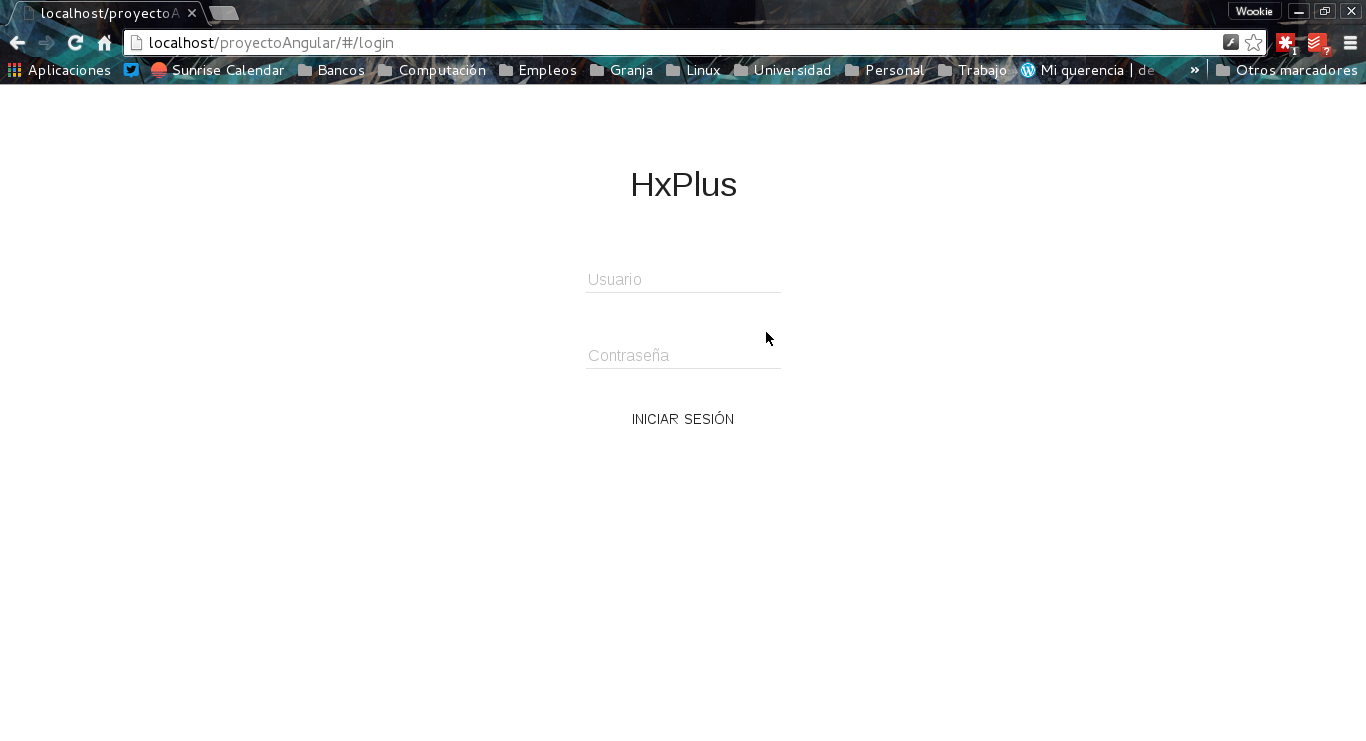
\includegraphics[width=.8\textwidth]{figures/p1}
                \end{center}
                \caption{Pantalla de Autenticación de usuarios}
                \label{Autenticación}
            \end{figure}
            
            Para ello se agregó al ``pom.xml" las dependencias requeridas para la autenticación. Ver cuadro \ref{artefactos-tba}
            
            \begin{table}[h!]
                
                \begin{center}
                    \begin{tabular}{|l|l|l|}\hline
                        Grupo & Artefacto & Versión \\\hline
                        io.jsonwebtoken & jjwt & 0.5.1 \\\hline
                    \end{tabular}
                \end{center}
                
                \caption{Artefactos de Maven: Autenticación}
                \label{artefactos-tba}
            \end{table}
            
            \item Se implementó el módulo de gestión de usuarios, en el mismo, un usuario, con las credenciales adecuadas, puede crear, usuarios nuevos y se despliega una lista de los usuarios en la  cual se puede elegir uno para luego poder editarlo o eliminarlo definitivamente de la base de datos. Esta última acción no es reversible por lo cual queda a consideración del \textit{Product Owner} si quedará finalmente la funcionalidad al alcance de los usuarios. Ver figuras \ref{Revisión} y \ref{Edición}.
            
            \begin{figure}[htbp!]
                \begin{center}
                    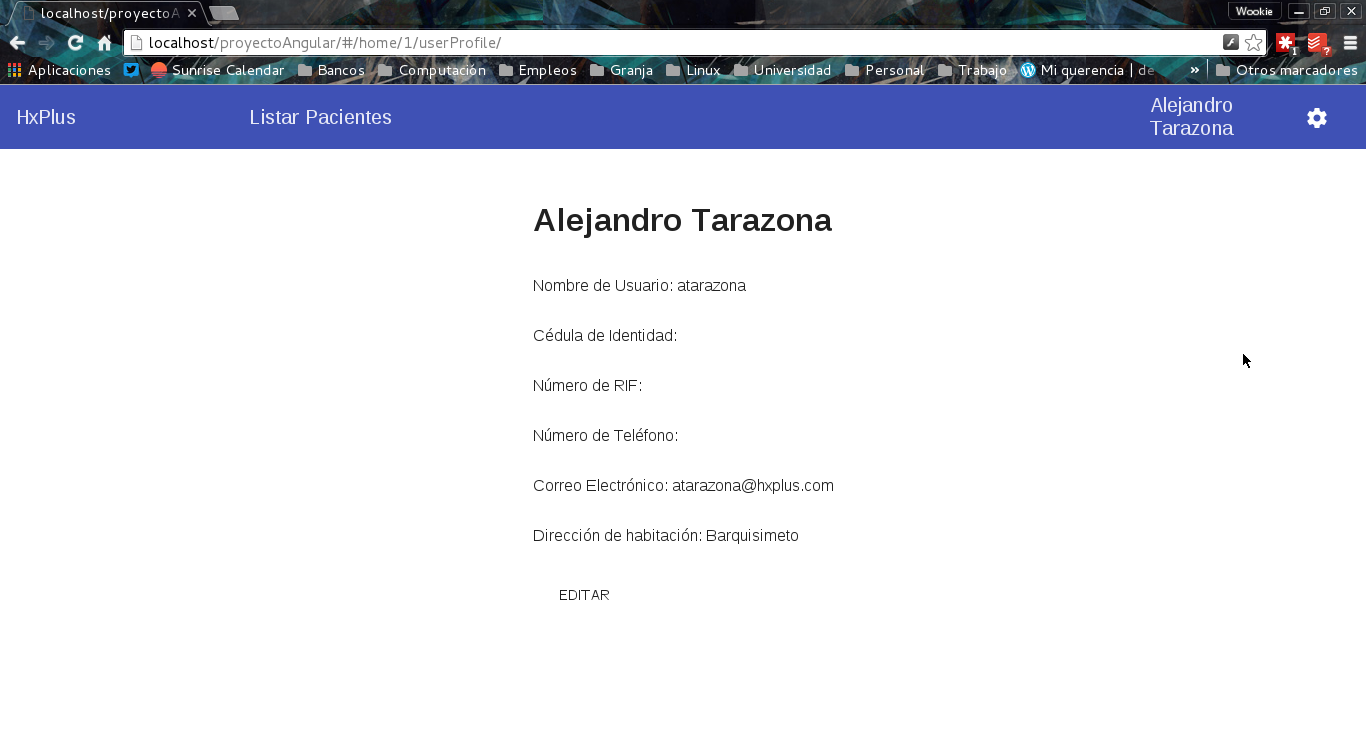
\includegraphics[width=.8\textwidth]{figures/p3}
                \end{center}
                \caption{Pantalla de Revisión de Usuario.}
                \label{Revisión}
            \end{figure}
            
            \begin{figure}[htbp!]
                \begin{center}
                    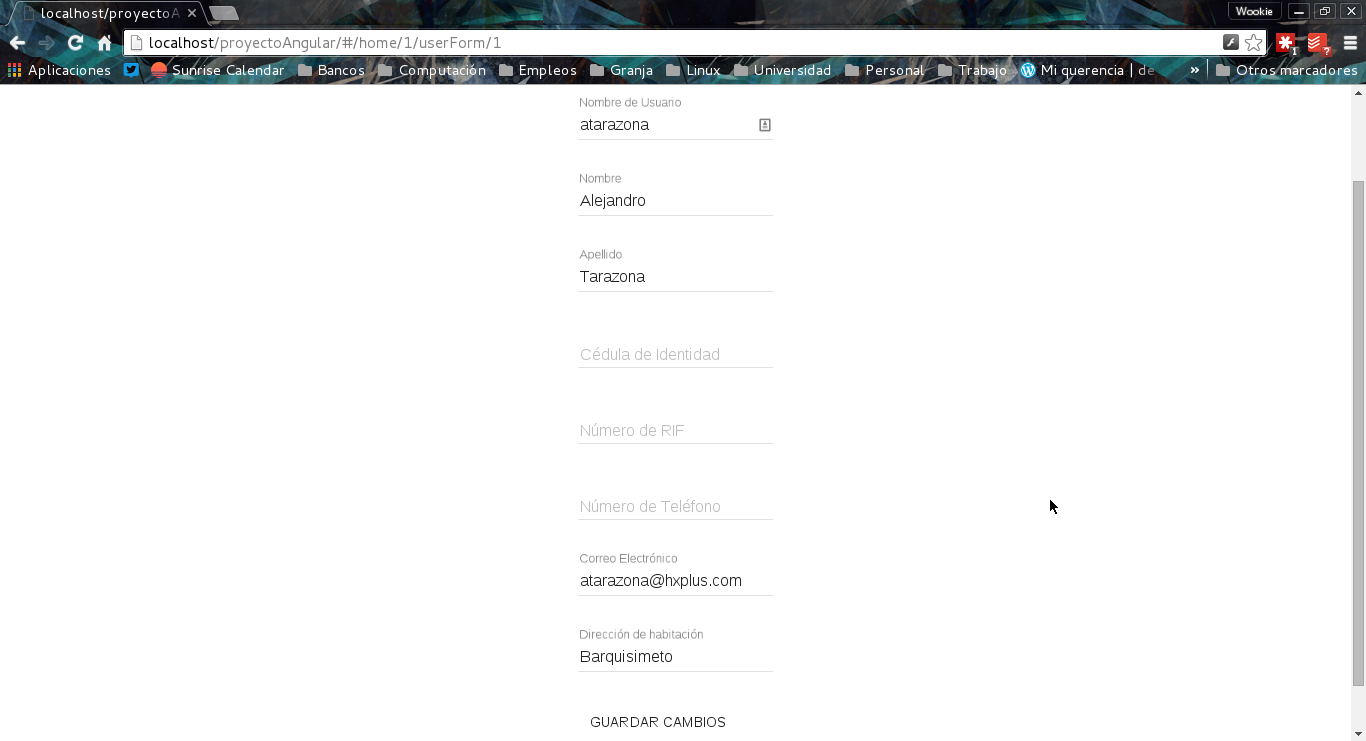
\includegraphics[width=.8\textwidth]{figures/p5}
                \end{center}
                \caption{Pantalla de Edición de Usuario.}
                \label{Edición}
            \end{figure}
            
        \end{itemize}
         

         
            
    \end{enumerate}
             
        
    \subsection{Cuarto Sprint: Consultas de Usuarios y Vista del doctor}
    
    En este \textit{sprint} se mejoró la estética de la lista de usuarios y se implementó la visualización de parte de los doctores.
    
    \begin{enumerate}
        \item Objetivos
        \begin{itemize}
            \item Consultas del módulo de usuarios.
            \item Desarrollo de la vista del doctor.
        \end{itemize}
        \item Actividades
        \begin{itemize}
            \item Ordenamiento de las listas de usuarios
            
            La lista de usuarios implementada en el \textit{sprint} anterior fue reordenada para aparecer alfabéticamente en pantalla. Las funcionalidades previas no fueron modificadas.
            
            \item Visualización de usuarios
            
            La lista también fue modificada para que fuese visualizada con apariencia de lista de usuarios siguiendo los lineamientos de Material Design. Ver figura \ref{Pacientes}.
            
            \begin{figure}[htbp!]
                \begin{center}
                    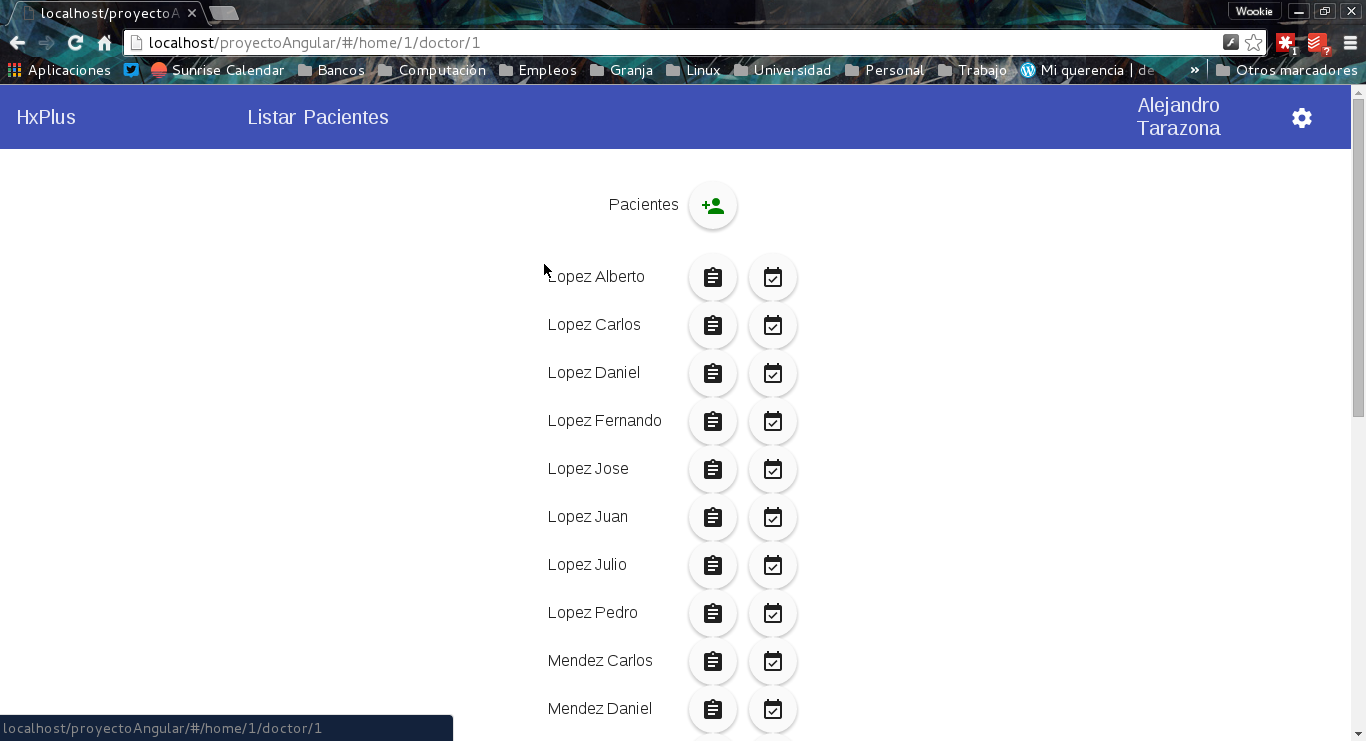
\includegraphics[width=.8\textwidth]{figures/p6}
                \end{center}
                \caption{\label{Pacientes}Lista de Pacientes del Médico}
            \end{figure}
            
            \item Creación de la vista del doctor
            
            Esta incluye la lista de pacientes a atender en el día actual y la lista de pacientes que ha atendido el doctor. Junto con las funcionalidades de:
            
            \begin{itemize}
                \item Agregar Paciente: Agrega un paciente nuevo a la lista de doctor, ya sea tomado de la lista de pacientes (Tal como se muestra en la figura \ref{Agregar}) o creando un nuevo historial y agregándolo inmediatamente a la lista de pacientes del doctor (Figura \ref{creación}).
                
                \begin{figure}[htbp!]
                    \begin{center}
                        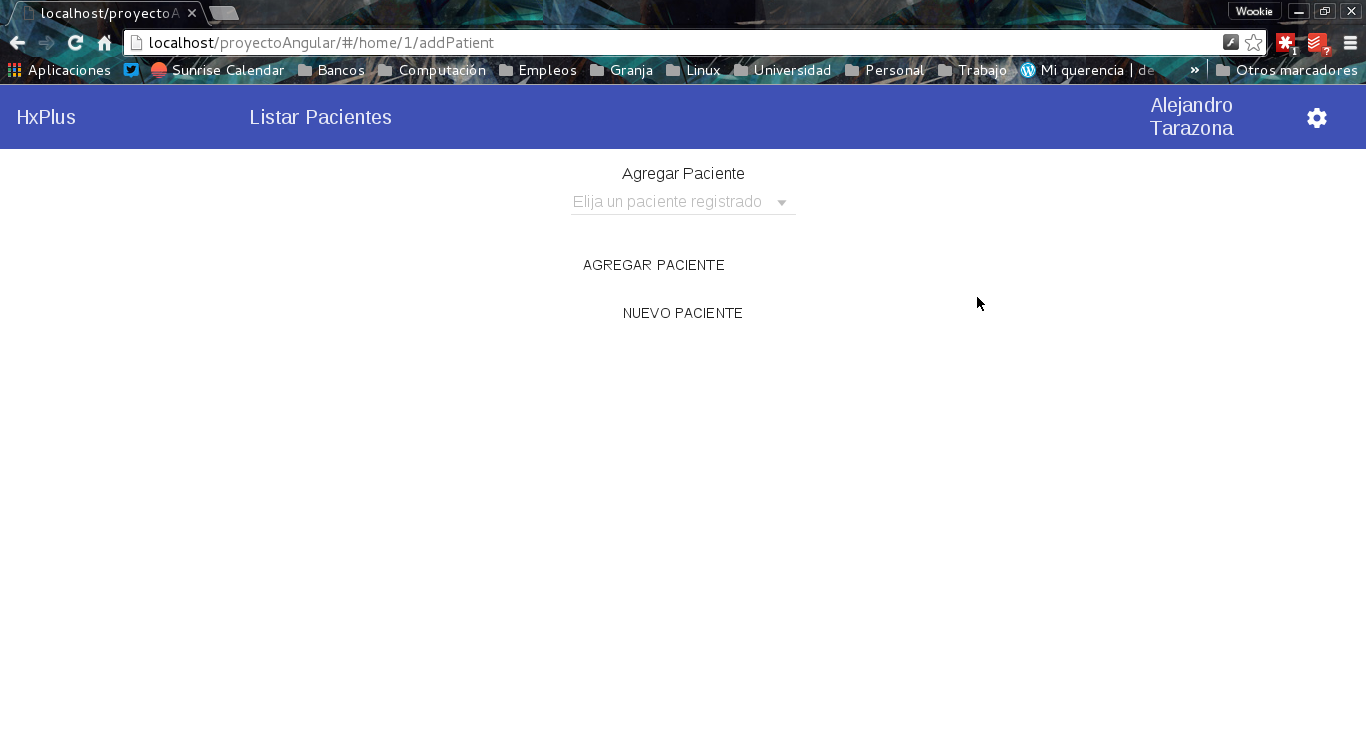
\includegraphics[width=.8\textwidth]{figures/p8}
                    \end{center}
                    \caption{Vista de Agregar pacientes que ya han sido atendidos por algún médico.}
                    \label{Agregar}
                \end{figure}
                
                \begin{figure}[htbp!]
                    \begin{center}
                        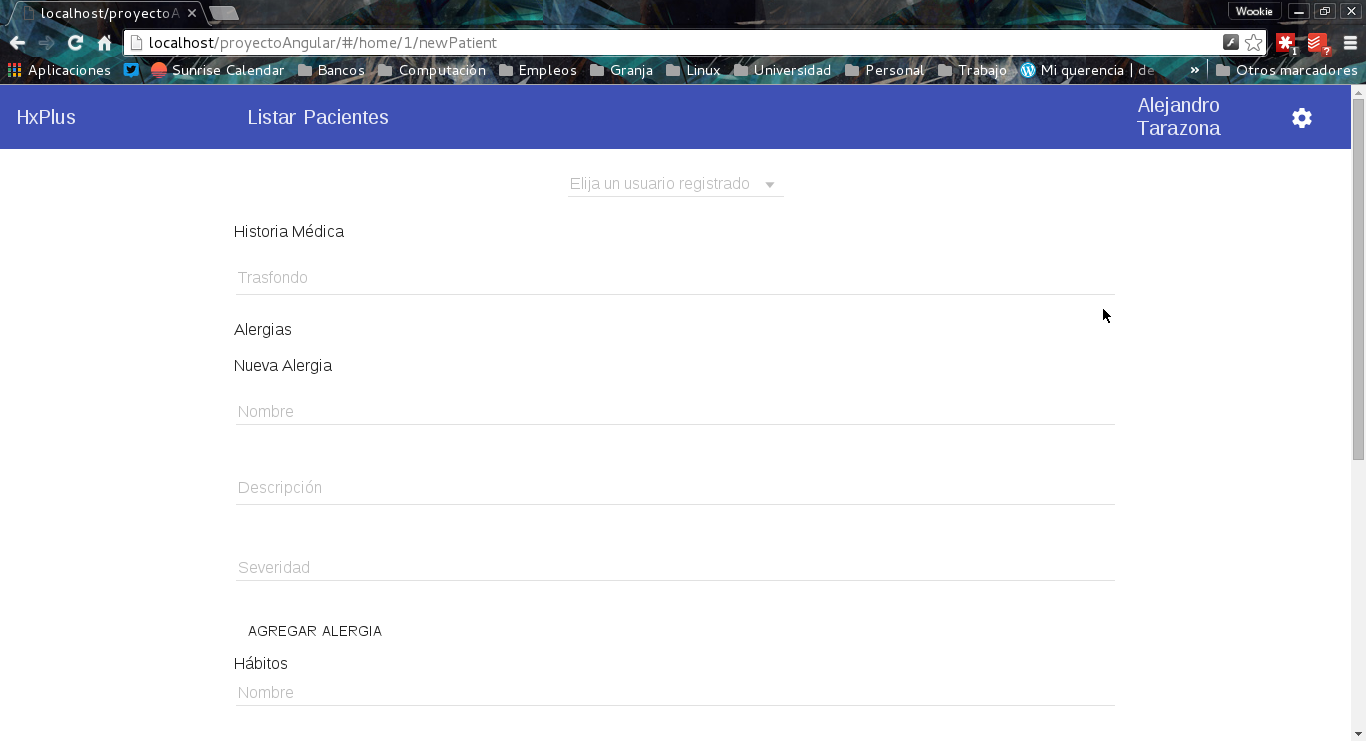
\includegraphics[width=.8\textwidth]{figures/p10}
                    \end{center}
                    \caption{Vista de creación de nueva historia médica para un paciente nuevo.}
                    \label{creación}
                \end{figure}
                
                \item Crear Consulta: Crea una nueva consulta al historial de paciente. En este \textit{sprint} se realizó la funcionalidad de ``programar" una confulta futura, que permitirá la planificación de consultas. Se dejó para un futuro \textit{sprint} la ceración de la consulta en sí misma ya que amerita el manejo de otros tipos de datos adicionales.
            \end{itemize}           
            
            No se implementó la funcionalidad de ``Eliminar Paciente" ni la de ``Modificar Paciente" dado que el sistema busca mantener un registro histórico de las consultas y un médico no debería poder modificar ni eliminar dicho registro, sólo agregar nueva información al mismo.
            
        \end{itemize}

    \end{enumerate}
        
        
    \subsection{Quinto Sprint: Consulta del Paciente}
    
    En este \textit{sprint} se implementó el módulo de consultas del paciente, en este módulo el doctor puede crear y almacenar los datos pertinentes a una consulta dada y los mismos serán agregados al historial médico del paciente.
    
    \begin{enumerate}
        \item Objetivos
        \begin{itemize}
            \item Generación de consultas.
            \item Gestión de la linea de tiempo de la consulta del paciente.
        \end{itemize}
        \item Actividades
        \begin{itemize}
            \item Crear consulta nueva
            
            Se crea la nueva consulta, permitiendo a médico almacenar los datos pertinentes. La consulta creada se agrega inmediatamente al historial del paciente, anexando los diagnósticos, en caso de haberlos, a su apartado exclusivo dentro del historial.
            
            Se almacenan los signos vitales o parámetros fisiológicos pertinentes, peso, estatura, tensión arterial entre otros. Se deja libertad al médico para añadir nuevos parámetros a los que ya estén almacenados en la base de datos (Figura \ref{parametros}).
            
            \begin{figure}[htbp!]
                \begin{center}
                    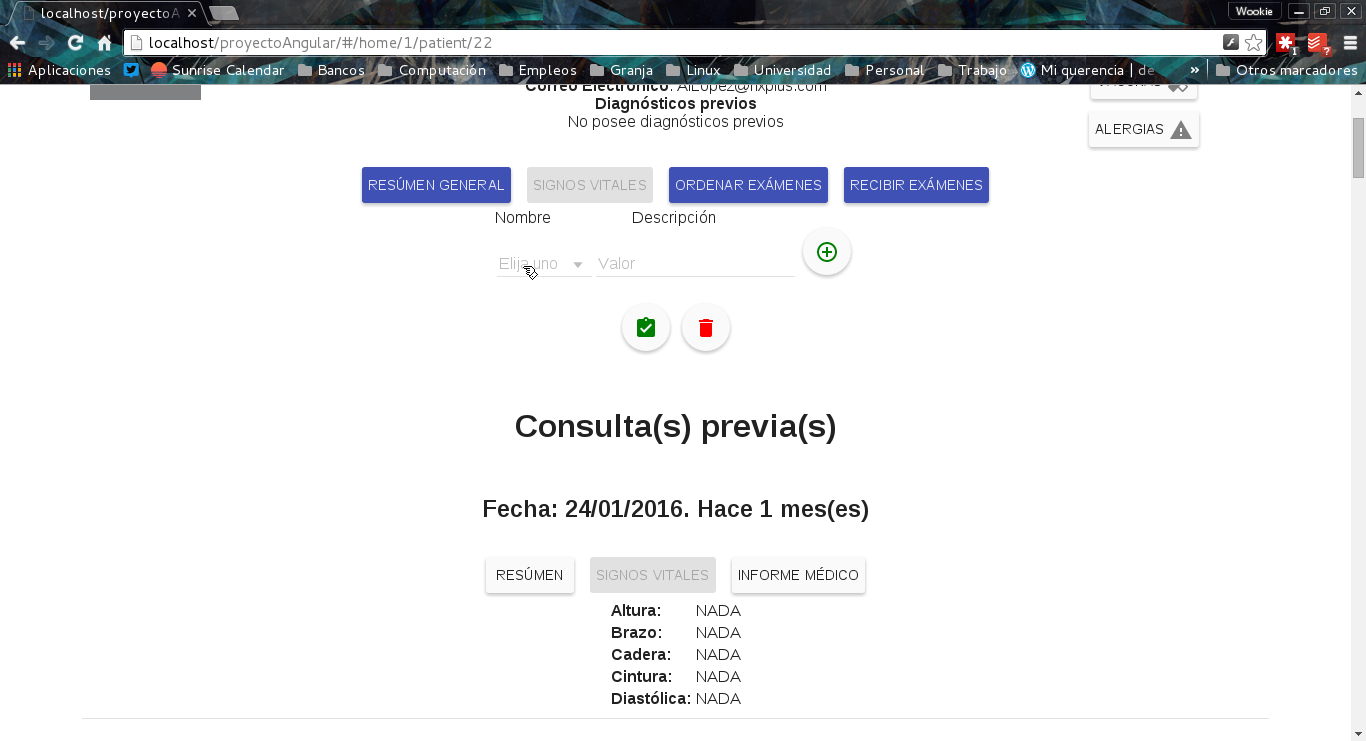
\includegraphics[width=.8\textwidth]{figures/p13}
                \end{center}
                \caption{\textit{Paarámetros Fisiológicos}}
                \label{parametros}
            \end{figure}
            
            \item Creación de \textit{Soap Note}
            
            Se crea y almacena, para cada consulta, los datos recogidos en la consulta (Figura \ref{soapnote}). Tales son:
            
            \begin{itemize}
                \item \underline{Subjetivos (\textit{Sbjective}):} Lo que el paciente atestigua, sintomas y comentarios hechos por el paciente en el lenguaje que el mismo paciente los exprese para así mantener la información sin cambios en caso de que sea necesario revisarlos.
                \item \underline{Objetivos (\textit{Objective}):} Lo que el médico puede observar en la consulta. Se usa en esta sección el lenguaje técnico propio de la medicina.
                \item \underline{Comentarios (\textit{Assessment})}: Algún comentario u obsevación adicional que pueda hacer el doctor.
                \item \underline{Plan:} Se acordó que el \textit{Plan} estaría en un apartado especial por cuestiones de simplicidad y acceso a los datos.
            \end{itemize}
            
            \begin{figure}[htbp!]
                \begin{center}
                    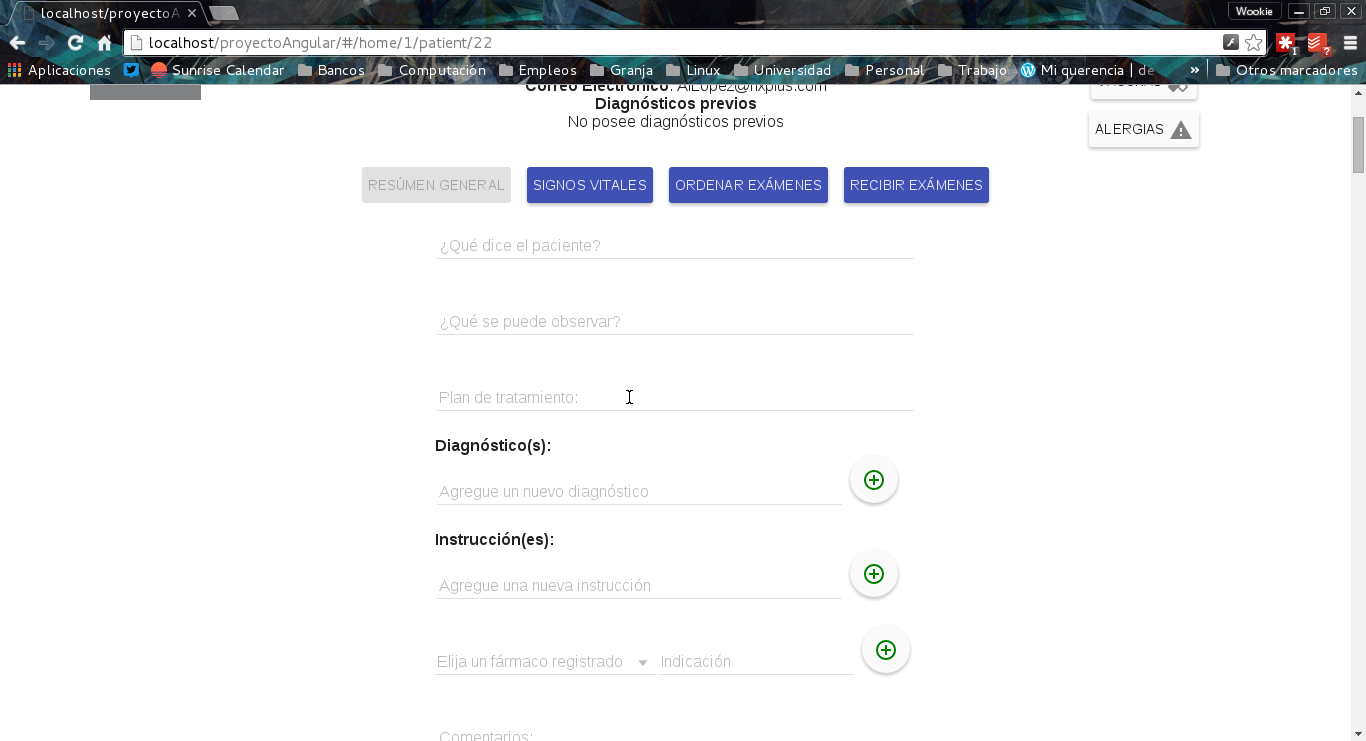
\includegraphics[width=.8\textwidth]{figures/p12}
                \end{center}
                \caption{\textit{Soap Note}}
                \label{soapnote}
            \end{figure}
            
            \item Solicitud y recepción de exámenes médicos
            
            El médico  tratante tiene uns sección de solicitud de exámenes médicos. En ella indica el nombre del exámen a solicitarle al paciente (Figura \ref{solicitudExamen}) Estas solicitudes quedan almacenadas y en futuras consultas, el médico tiene la opción de indicar la recepción de algún exámen previamente solicitado, ya sea uno o varios de ellos (Figura \ref{recepcionExamen}).
            
            \begin{figure}[htbp!]
                \begin{center}
                    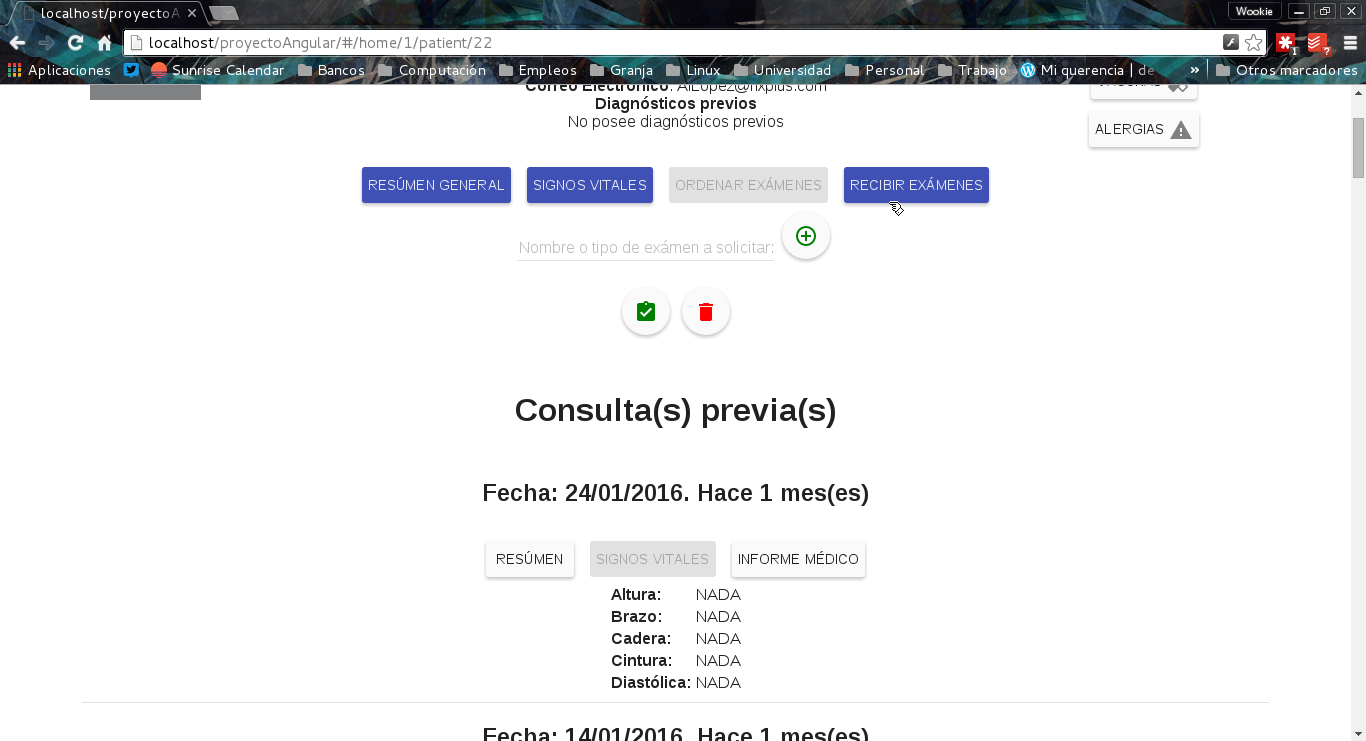
\includegraphics[width=.8\textwidth]{figures/p16}
                \end{center}
                \caption{\textit{Solicitud de Exámenes}}
                \label{solicitudExamen}
            \end{figure}
            
            \begin{figure}[htbp!]
                \begin{center}
                    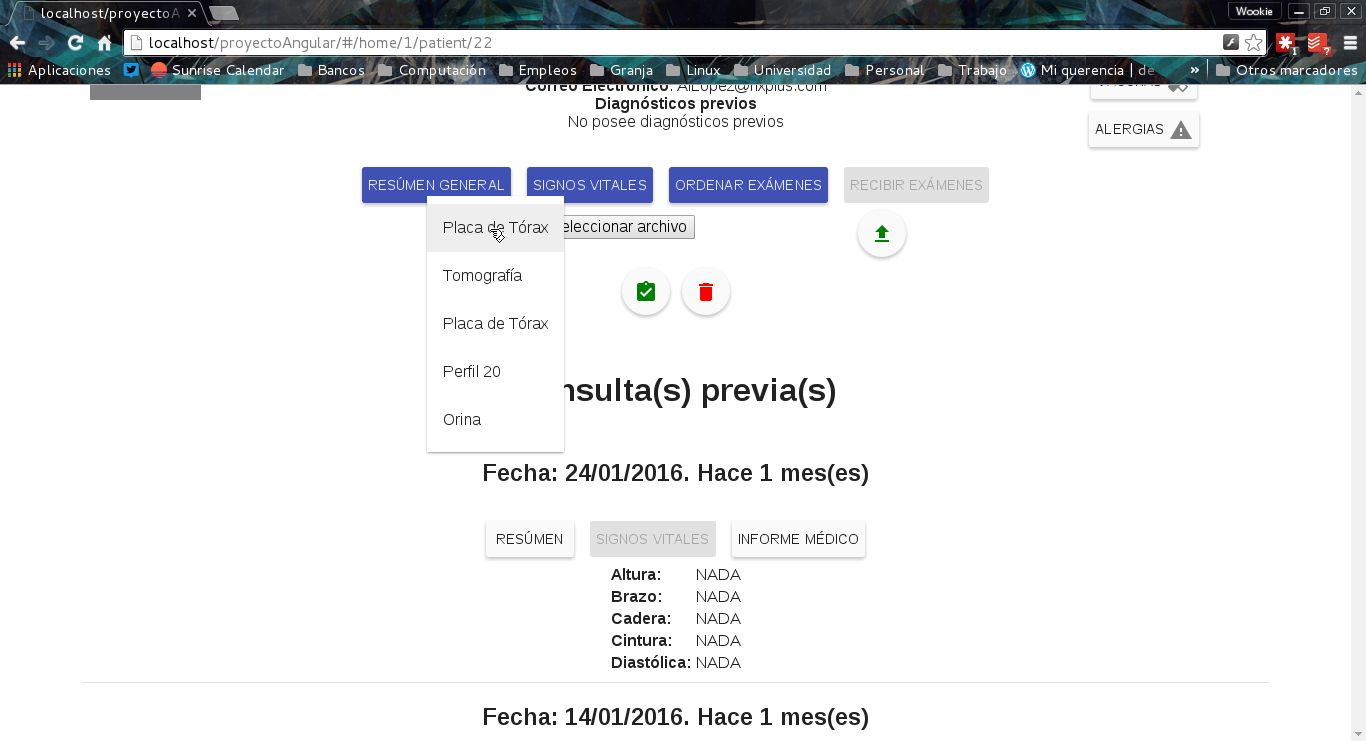
\includegraphics[width=.8\textwidth]{figures/p17}
                \end{center}
                \caption{\textit{Recepción de Exámenes}}
                \label{recepcionExamen}
            \end{figure}
            
            En la sección de recepción de exámenes, el médico también tiene la opción de adjuntar algún archivo, ya sea resultados (en el caso de exámens sanguíneos) o imágenes (ecografías, rayos X, etc) los cuales serán anexados a la respectiva consulta y con ella al historial del paciente.
            
            \item Creación de diagnósticos
            
            El médico también puede almacenar uno o varios diagnósticos por consulta, estos constan de un nombre de enfermedad o dolencia y una gravedad. Ello lo elige de listas desplegables que estarán a su disposición tomando la base de datos del sistema. También se le permite agregar un nuevo diagnóstico en caso de carecer de ello el sistema, y el mismo será almacenado con posibilidad de reutilización (sólo del nombre) en futuras consultas.
            
            \item Creación del plan de tratamiento
            
            El médico puede crear un plan de tratamiento, el cual consiste en:
            \begin{itemize}
                \item Recomendaciones: Cambios o hábitos de los que el paciente deba cuidarse, así como recomendaciones alimenticias y reposos. Es una sección informal.
                \item Comentarios: Algun comentario extra, preguntas o anotaciones que el médico quiera hacer del conocimiento del paciente.
                \item Tratamiento: Este incluye al menos un medicamento y la posología elegida para cada uno de los medicamentoa añadidos. Los medicamentos son elegidos de la base de datos del sistema. El administrador del sistema se encararía de añadir o eliminar medicamentos a la base de datos por ahora.
                \item Récipe Médico: En este se indica un medicamento y su respectiva dosis para permitir al paciente su compra en la farmacia de su preferencia.
            \end{itemize}
            
            Esta información estará disponible, en un futuro \textit{Sprint} para ser impresa en hojas, según el formato lo establezca, y ser entregada al paciente.
            
        \end{itemize}
    \end{enumerate}
        
        
    \subsection{Sexto Sprint: Generar informes}
    \begin{enumerate}
        \item Objetivos
        \begin{itemize}
            \item Generación de informes médicos y reposos.
        \end{itemize}
        \item Actividades
        \begin{itemize}
            \item Investigar las herramientas disponibles para generar archivos PDF.
            \item Evaluar la compatibilidad con las herramientas y el \textit{framework} que se está usando en el dessarrollo de \textit{HxPlus Ocupacional}.
            \item Elegir una de las herramientas y realizar los cambios adecuados para su uso en el sistema. Para \textit{HxPlus Ocupacional} se eligión iText por las razones mencionadas anteriormente.
        \end{itemize}
    \end{enumerate}
        
    \subsection{Septimo Sprint: Generar informes}
    \begin{enumerate}
        \item Objetivos
        \begin{itemize}
            \item Vista de Solicitud de informes.
        \end{itemize}
        \item Actividades
        \begin{itemize}
            \item Se implantó la vista de solicitud de informes médicos con posibilidad de selección múltiple. Los parámetros son:
            \begin{itemize}
                \item Examen físico
                \item Diagnóstico(s)
                \item Tratamiento
                \item Comentario(s)
            \end{itemize}
            
            Tal como se muestra en la figura \ref{solicitudInforme}. Esto permite que en un solo formulario, el médico tiene la posibilidad de generar tanto informes como reposos médicos.
            
            \begin{figure}[htbp!]
                \begin{center}
                    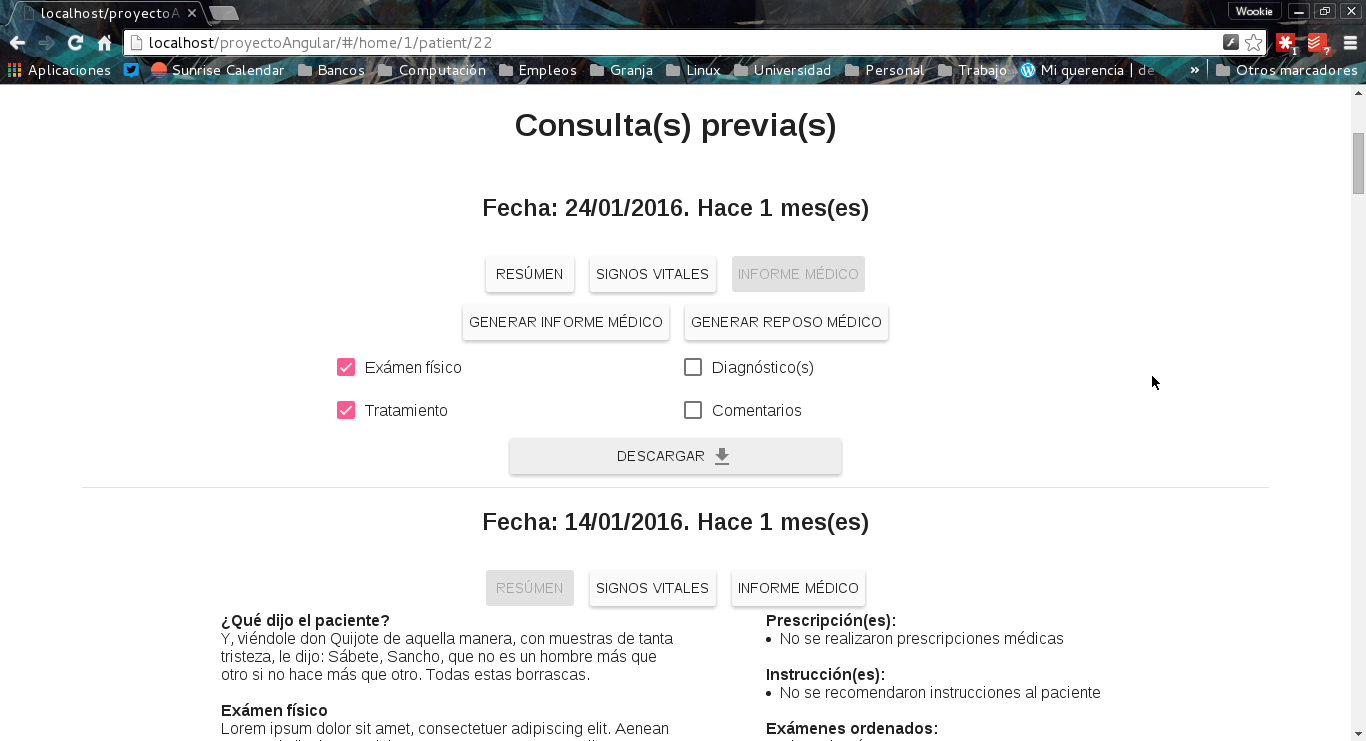
\includegraphics[width=.8\textwidth]{figures/p23}
                \end{center}
                \caption{Sección de solicitud de informes médicos.}
                \label{solicitudInforme}
            \end{figure}
        \end{itemize}
    \end{enumerate}
        
        
    \subsection{Octavo Sprint: Generar informes}
    \begin{enumerate}
        \item Objetivos
        \begin{itemize}
            \item Generacion de informes.
        \end{itemize}
        \item Actividades
        \begin{itemize}
            \item Se implantó el módulo de generación de informes médicos, tal y como fue descrito anteriormente, usando los parámetros selecciónados se generó el informe respectivo usando el formato indicado. Ver figura \ref{informeModelo}.
        \end{itemize}
        
        \begin{figure}[htbp!]
            \begin{center}
                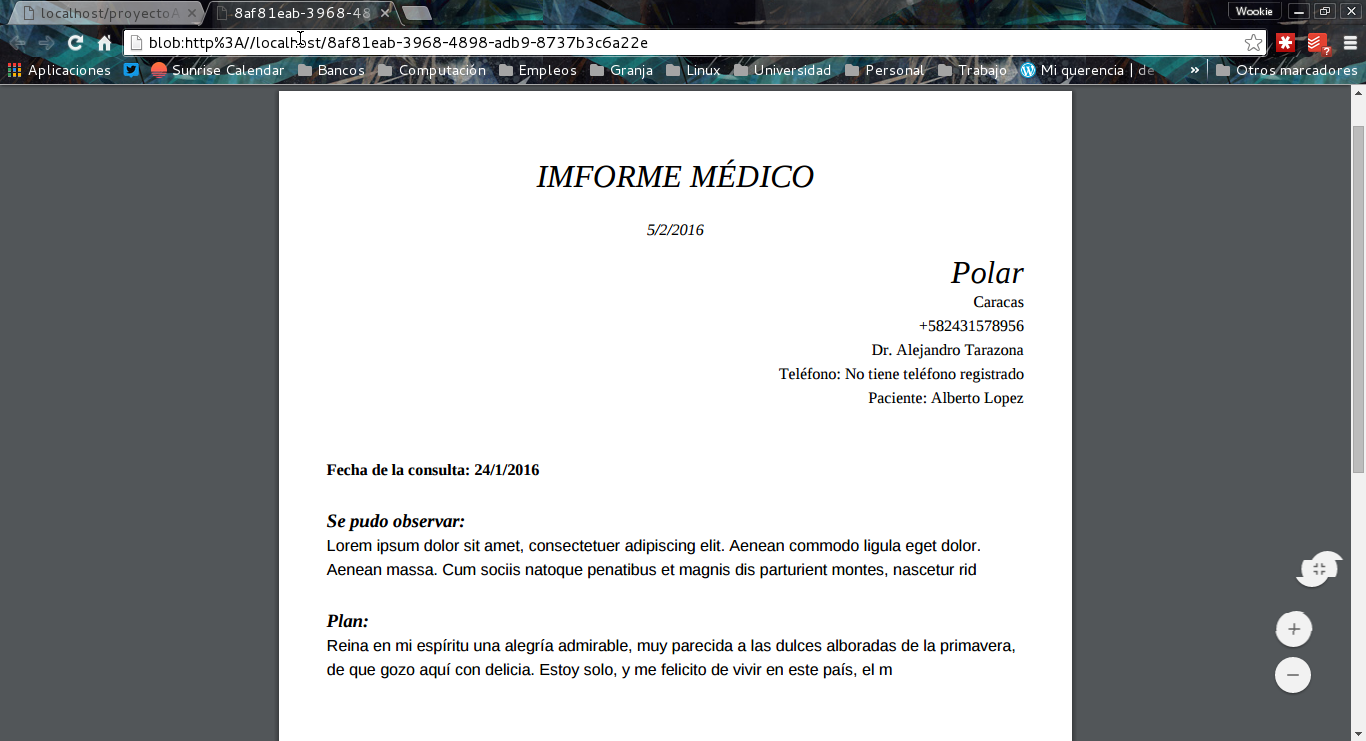
\includegraphics[width=.8\textwidth]{figures/p22}
            \end{center}
            \caption{Informe modelo}
            \label{informeModelo}
        \end{figure}
    \end{enumerate}
        
    
\section{Fase de Cierre}
    \subsection{Primer Sprint: Pruebas finales y puesta en producción}
    \begin{enumerate}
        \item Objetivos
        \begin{itemize}
            \item Resolución de incidencias.
            \item Diseño y ejecución de pruebas.
            \item Puesta en producción.
        \end{itemize}
        \item Actividades
        \begin{itemize}
            \item Se revisaron las incidencias y posibles errores de consistencia de la información y su acceso en el sistema.
            \item Se realizaron pruebas de aceptación de parte del \textit{Scrum Master} en el uso del sistema.
        \end{itemize}
    \end{enumerate}
        
    \subsection{Segundo Sprint: Redacción del libro de pasantías}
    \begin{enumerate}
        \item Objetivos
        \begin{itemize}
            \item Redacción del libro de pasantías.
            \item Revisión y culminación del libro de pasantías.
        \end{itemize}
        \item Actividades
        \begin{itemize}
            \item Se recopiló la información del proyecto
            \item Se realizó el filtrado de dicha información y se llevó al presente trabajo en limpio para su presentación.
        \end{itemize}
    \end{enumerate}
        
        
    \subsection{Dificultades generales encontradas}
    
    Las dificultades encontradas durante el desarrollo del proyecto fueron:
    
    \begin{itemize}
        \item \textbf{Restricción en el uso de herramientas:} el \textit{Product Owner} solicitó explícitamente el uso de Java, SPRING, Hbernate, JavaScript, MySQL, AngularJS y JSON, tal y como fue descrito, para el desarrollo. Lo cual, si bien facilitó la creación y desarrollo del proyecto, dejó imposibilitada la posibilidad de, con tecnologías actuales, dar soporte a una base de datos orientada a eventos, tal como se pretendía hacer en el principio, y no se logró este enfoque.
        
        \item \textbf{Falta de informción de parte de Inpsasel:} originalmente se buscaba generar informes médicos especializados para el reporte de enfermedades ocupacionales al Inpsasel, órgano encargado de la gestión de enfermedades ocupacionales en el émbito nacional. Sin embargo, la falta de información, formatos y, más adelante, el lanzamiento de su portal (de Inpsasel) con automatización de dicha gestión, dejó a HxPlus Ocupacional sin la necesidad de realizar dichos informes.
    \end{itemize}
    
    \subsection{Resultados Generales}
    
    El proyecto de pasantía se completó satisfactoriamente. A pesar de no poseer la funcioncionalidad de generación de informes de Inpsasel, la empresa de consideró satisfecha con los módulos implementados. La línea de tiempo de consultas se muestra adecuadamente y en orden cronológico, los diagnósticos y planes son almacenados y mostrados a gusto de la empresa y de conformidad con los lineamientos.
    
    Queda de parte de la empresa gestionar el desarrollo de futuros módulos o funcionalidades para la aplicación.
    
    
    
\pagebreak
     \chapter{Conclusiones y Recomendaciones}

    Habiendo terminado el proyecto, se logró la implementación del sistema ``HxPlus Ocupacional" para Globisoft S.A. apoyando de esta manera su misión de brindar apoyo tecnológico al área médica en Venezuela. El mercado actual de herramientas en este ámbito está en su fase inicial y, aunque hay resistencia al cambio por parte de los médicos nacionales, la familiaridad y una interfaz planificada para la usabilidad, ayudará a que las nuevas generaciones hagan uso de este sistema.
    
    SCRUM permitió una organización rápida y la debida evaluación oportuna de los objetivos logrados y la planificación de la siguiente serie de objetivos, adaptándose así a los inconvenientes evidenciados.
    
    El proyecto, si bien orientado a medicina ocupacional, se recomienda en un futuro, incluir también el área farmacéutica y su integración con ``HxPlus", el cual se encuentra en funcionamiento. Con esto se crearía un sistema distribuido integral de gestión de consultas, remisión de informes médicos y generación de constancias, informes y récipes médicos y que a su vez le permita a las empresas farmacéuticas publicidad y registros en tiempo real, a los pacientes, tener siempre a su disposición los planes de tratamiento, récipes médicos, los diagnósticos realizados y su historial médico en caso de alguna eventualidad como pérdida del mismo u olvidos ocasionales.
    
    También, y en el marco de las tecnologías usadas, se sugiere una evaluación del patrón de almacenamiento de la base de datos ya que el uso de un patrón orientado a eventos podría ser provechoso al momento de recuperación de fallos dentro de la base de datos.


    
   
     \addcontentsline{toc}{chapter}{Anexos}
\chapter*{Anexos}

\addcontentsline{toc}{section}{Anexo A: Diagrama ER-E y Glosario de términos}
\section*{Anexo A: Diagrama ER-E y Glosario de términos}
            \begin{figure}
                \begin{center}
                    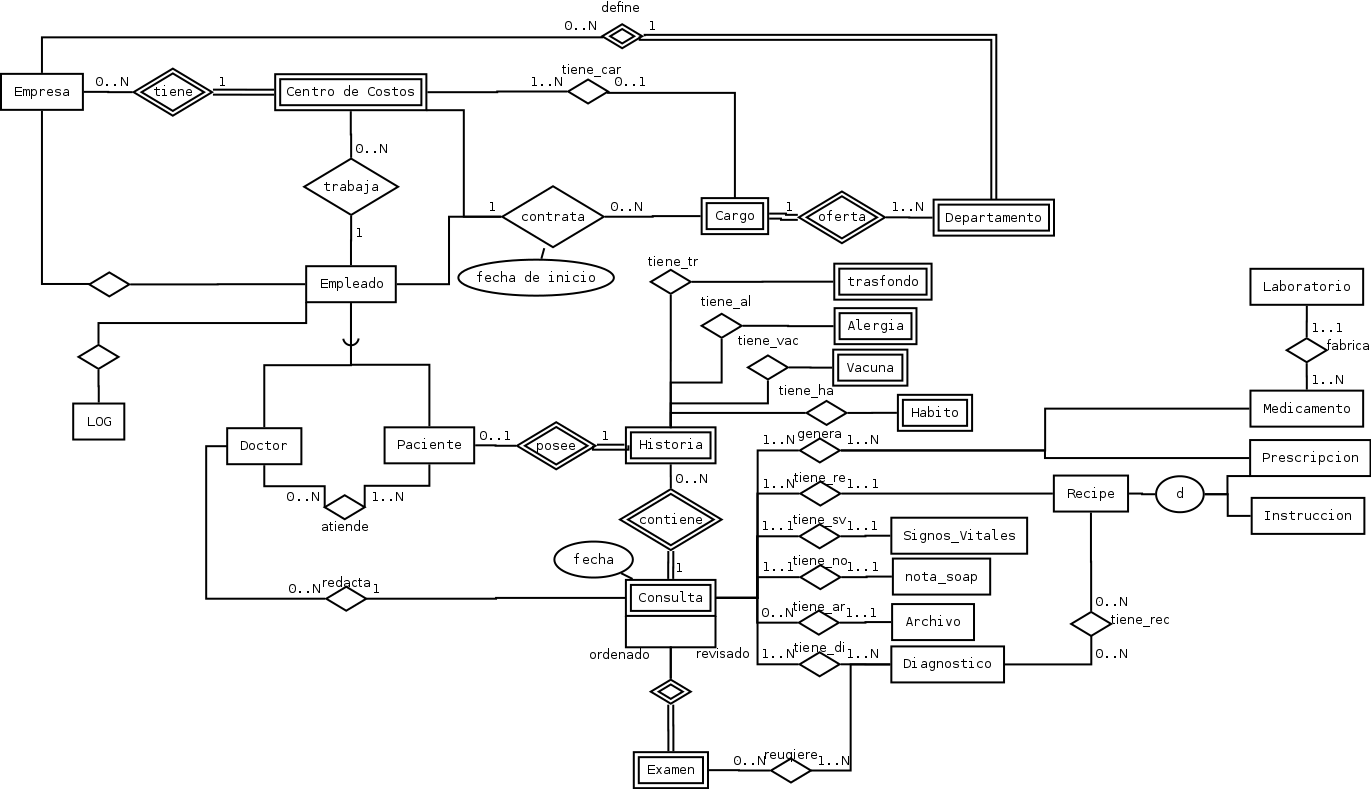
\includegraphics[scale=.45,angle=90]{figures/DiagramBD}
                \end{center}
                \caption{Diagrama ER-E de la base de datos.}
            \end{figure}

\pagebreak
    % Diagrama CU
    % Diagrama Clases
    % Diagrama ER-E <----Listo
    % Screenshots
    % DAS(?)
     \addcontentsline{toc}{chapter}{Bibliografía}
\printbibliography
\pagebreak
     
\end{document}